\chapter{Introduction}
\begin{blueshaded}
bla bla bla
\end{blueshaded}

% -------------------------------
% -------------------------------
%
%     RESEARCH CONTEXT
%
% -------------------------------
% -------------------------------

\color{gray}
--- Introduire la notion de brain states ---\\
\citep{poulet_cortical_2019}:\\
"Even in the absence of any external sensory input or motor activity, the brain is constantly active. This ongoing, or spontaneous, electrical activity was first revealed in living animals by Caton (1875) and then by Berger (1929) in humans using electroencephalography (EEG) recordings on the skull surface. Hans Berger’s classical EEG recordings from the occipital cortex of awake, but relaxed, subjects with their eyes closed showed high-amplitude oscillatory activity around 10–15 Hz that transitioned rapidly to smaller and faster fluctuations whenever the subject opened his eyes or performed mental calculations. This pioneering work was the first report of a brain state change correlated with a change in behavioral or mental state. It also introduced the notion of brain rhythms or oscillations, and the idea that different brain states could be characterized by the dominant frequency component of the EEG activity"
\color{black}




\newpage
% -------------------------------
% -------------------------------
%
%     TOOLS/BACKGROUND IN NEUROSCIENCE
%
% -------------------------------
% -------------------------------
\section{Background in neuroscience}


% -----------------------------------
%       Anatomy: brain & structures
% -----------------------------------
\subsection{Neuroanatomy}
Our brain is the organ that controls our motor skills, our memory, our emotion, our breathing or every process that governs our body and our mind. It receives and emits chemical and electrical signals throughout our body to react to the external world, to drive our behavior and to build our conscious. This organ is divided in several structures performing different functions. For example, the \textit{cortex} is the outer part of the brain and is responsible for a variety of functions including movement, emotion, sensory perception among others. . The main part of the cortex is the \textit{neocortex} and the rest is called allocortex. Cortical neurons are organized in the horizontally in six layers and in the radially in column. It is divided in different regions associated with a different functions. For example, the frontal cortex is involved in decision-making while the occipital cortex processes visual information. The \textit{thalamus} is  located deep in the brain and acts as a relay station for sensory information. It receives signal from the body and sends them to the appropriate region in the cortex. It is involved in regulating consciousness, sleep and arousal. The \textit{hippocampus} is a seahorse-shaped structure located in the temporal lobe of the brain and is primarily involved in the formation and consolidation of memories. It is also involved in spatial navigation, which is the ability to navigate and remember the locations of objects in our environment. This thesis briefly mentions several structures crucial to understanding the brain's functioning, such as the basal ganglia, striatum, brainstem, locus coeruleus, basal forebrain, nucleus basalis of Meyner, amygdala, raphe nuclei, substantia nigra, ventral tegmental area, and hypothalamus. Like the components of a factory, these structures are interconnected and work together to sustain life. A deficiency in any of these parts can lead to pathological behaviors and disrupt the brain's proper functioning. Therefore, studying the neuroanatomy and coordination between these structures has been crucial in developing therapeutic solutions.
 




\begin{figure}[h!]
    \centering
    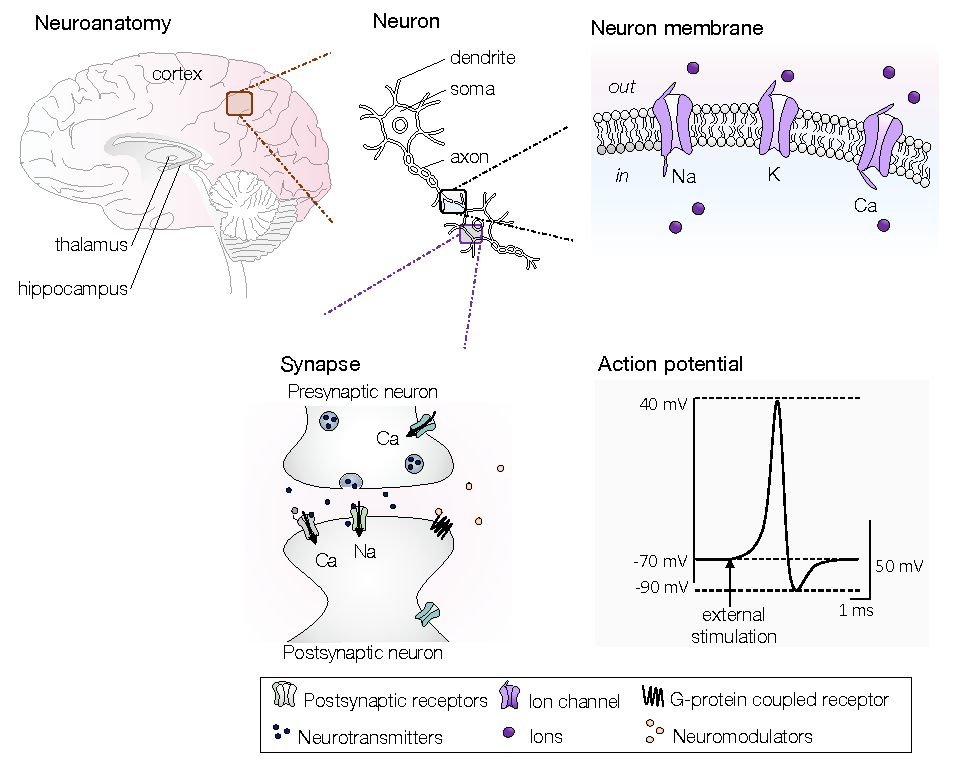
\includegraphics{latex/fig/Intro/Bgd_scale.pdf}
    \caption{Caption}
    \label{fig:Bgd_scale}
\end{figure}

% -----------------------------------
%       Neurons
% -----------------------------------
\subsection{The basics of neuron structure and function}
Our brain is composed of more than 86 billion of neurons \citep{Herculano-Houzel_human_2009}. These fundamental units process the information between the body and the brain. Neurons are excitable that are activated by chemical or electrical signals, and they communicate with one another by generating electrical signals known as \textit{action potential}. Each neuron consists of three main parts: the \textit{dendrite}, which collects the incoming signals, the \textit{soma}, known as the cell body, which integrates these signals and the \textit{axon}, which transmits the response. 

Neurons share similar components with classical cells such as the plasma membrane that separates the intra- and extracellular compartments. This membrane is permeable to small molecules and water, but almost fully impermeable to ions and large molecules. \textit{Ion channels}, which are particular proteins embedded in the membrane, allow the flow of ions through the membrane. They are selective to a given type of ions such as sodium (Na$^+$), potassium (K$^+$), calcium (Ca$^{2+}$) or chloride (Cl$^-$) and they regulate the concentration of these ions accross the membrane. Therefore, the concentration of positive and negative ions on both sides of the membrane and its permeability generate an electrical potential called the \textit{membrane potential}. Without any external signal, the neuron is at its resting potential around \SI{-70}{mV}, which is maintained by the balance of ion concentration and ion channel activity. 

When a neuron receives a stimulus such as stress, pressure, electrical current or chemical transmitters, ion channels open, allowing the flow of ions through the membrane, causing a change in the potential. The neuron responds to this change, by altering its membrane potential. A positive stimulus is increasing the potential, known as \textit{depolarization}, while a negative stimulus decreases the potential, known as \textit{hyperpolarization}. A sufficient depolarization from the resting potential causes the all-or-nothing rise in the membrane potential, corresponding to the \textit{action potential} or \textit{spike}. This also reflects the cell excitability.

% -----------------------------------
%       Ion channels
% -----------------------------------
\subsection{Ion Channels: Their Structure and Role in Neuron Excitability}
Ion channels are membrane proteins that allow the flow of ions following gradient concentration. For example, ions channels allowing calcium flow are called calcium channels. These gateways have specific opening and closing mechanisms that are regulated by complex processes. They can be dependent on the membrane voltage or the calcium concentration. They open or close at different timescales. They can also have blockers that are dependent on other factors. Their kinetics are critical in the regulation of the membrane potential and govern the neuron excitability. Ion channels are complex transmembranic proteins with several substructures that allow the channel opening and closing. These substructures can be described at a more abstract level by visualizing the ion channel with gates; an activation gate or a inactivation gate. Neurons can produce a variety of response thanks to the interplay between the different ion channels that have various gating kinetics and voltage-dependency.


% -----------------------------------
%       Action potential
% -----------------------------------
\subsection{The mechanism of action potential generation}
The most familiar neuronal response is the action potential. At rest, the membrane potential is around \SI{-70}{mV}. When the neuron receives an excitatory stimulus, it depolarizes. If the input stimulus is weak, the neuron will go back to its resting state. If the stimulus is strong, it is activated the choreography of ion flows that builds up the action potential. Sodium channels are voltage-dependent. They allow sodium ions to enter that further depolarize the membrane voltage. Due to the voltage-dependency, more ions are entering and it causes a positive feedback. It creates a rapid depolarization known as the rising phase of the action potential. As the membrane reaches its peak, the voltage-dependent potassium channels open allowing potassium to exit the cell. This repolarizes the neuron on a slower timescale and brings it back to its resting value. The membrane voltage becomes slightly more hyperpolarized than its resting state called the hyperpolarization before it returns to its resting state thanks to the closing of ion channels and the activity of the ion pumps. 

This choreography is governed by the dynamics of sodium and potassium channels. At rest, sodium and potassium activation gates are closed and sodium inactivation gate is open. The excitatory stimulus causes the depolarization of the membrane voltage that causes the fast opening of the sodium activation gate resulting in sodium ion influx. The potassium activation gate is opening but on a slower timescale resulting in potassium ions release after several milliseconds. In parallel, the sodium inactivation gate slowly close stopping the sodium ion influx. The neuron hyperpolarizes causing sodium channel activation gate and potassium channel activation gate to close due to their voltage-dependency and sodium channel inactivation to open again. 

Now that the mechanisms of action potential generation is detailed, the remaining question is how this electrical signal is transmitted to other neurons. 


% -----------------------------------
%       Synapse
% -----------------------------------
\subsection{The Synapse: From Action Potential to Neurotransmitter Release}
When an action potential is generated at the soma, it propagates along the axon. It reaches the axon terminal called the \textit{synapse} and it triggers the release of chemical substances, called the neurotransmitters, to the target neurons. The electrical signal is transformed into a chemical signal. There also exist electrical synapse called gap junction but this thesis focuses on the chemical ones \citep{heidelberger_synaptic_2014}. 

The membrane is depolarized by the arrival of the action potential. It opens the voltage-gated ion channels, allowing calcium to enter the presynaptic neuron and to trigger a signalling cascade. Synaptic vesicles  fuse with the membrane of the presynaptic neurons and releases the stored neurostransmitters in the synaptic cleft. These neurotransmitters bind to the postsynaptic neuron receptors. It generates the opening or closing of these receptors translated by an increase or a decrease of the postsynaptic membrane potential that respectively define an \acrfull{EPSP} or an \acrfull{IPSP}. 
%\textcolor{gray}{Non-neuronal cells such as astrocytes, located near the synaptic cleft, contribute to the neurotransmitter wash-out or regulation \cite{heidelberger_synaptic_2014}}.\\


% -----------------------------------
%       NT & NMOD
% -----------------------------------
\subsection{Neuromodulation: from the definition to its essential and unsolved role in our brain}
\subsubsection{Neurotransmitters vs Neuromodulators: understanding the distinction}
\textit{Neurotransmitters} are chemical substances released by neurons to targeted neurons. There exist different types: \acrfull{NA}, also called norepinephrine, \acrfull{ACh}, \acrfull{5-HT}, \acrfull{DA}, \acrfull{HA} \acrfull{Glu} and \acrfull{GABA}. They target postsynaptic receptors in order to convey the electrochemical signal. In this way, they perform the synaptic transmission.

\textit{Neuromodulators} are a subset of neurotransmitters with a more diffuse release compared to the targeted action of the neurotransmitters during the synaptic transmission. Neuromodulators bind to G protein-coupled receptors and alter the cellular or synaptic properties of the neurons. Instead of carrying the information as performed by neurotransmitters, they can modulate the synaptic transmission by modifying the electrical behavior of the pre- or the postsynaptic neurons. 


\smallbreak
\noindent
\begin{minipage}{0.45\textwidth}
As a brief reminder, two main classes of receptors exist\citep{purves_neuroscience_nodate}. The \textit{ionotropic receptors}, also called called neurotransmitter-gated or ligand-gated channels,  directly open ion channels as soon as the neurotransmitter bind to the protein. The  \textit{metabotropic receptors} are membrane receptors that triggers a cascade of intracellular events using second messenger signal. They are indirectly linked to ion channel regulation.
\end{minipage}
\hfill
\begin{minipage}{0.45\textwidth}
    \begin{shaded}
        Fun fact sur l'histamine
    \end{shaded}
\end{minipage}


% -----------------------------------
%       NMOD: inventaire
% -----------------------------------
\subsubsection{Overview of Major Neuromodulators and their Functions in the Brain}
Neuromodulators play fundamental roles in our brain, and their actions are diverse. However, due to their diffuse effects, it can be challenging to identify their key functions. Moreover, they often work together, as demonstrated by research \citep{gu_neuromodulatory_2002, avery_neuromodulatory_2017, nadim_neuromodulation_2014}. The following is a brief, non-exhaustive overview of the main neuromodulators, categorized according to the location of their generating neurons, their projection regions, and their primary functions.

\begin{figure}[h!]
    \centering
    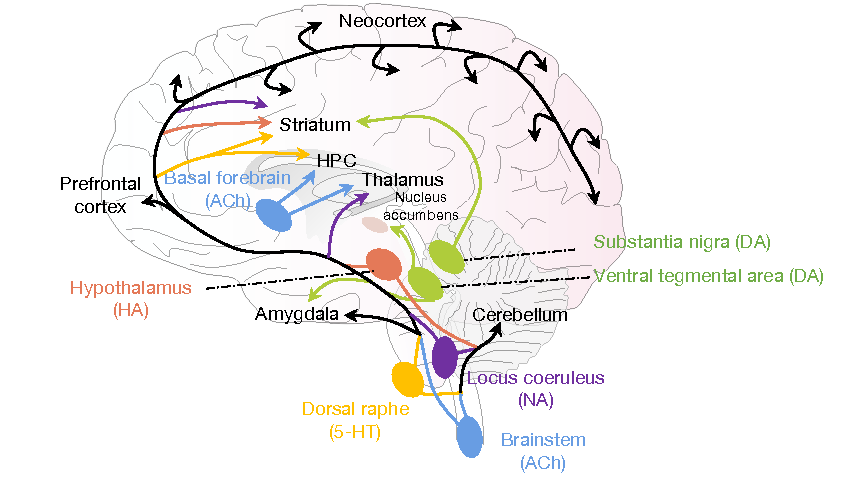
\includegraphics{latex/fig/Intro/Bgd_NMOD.pdf}
    \caption{Caption inspired from \citep{bear_neuroscience_2016, mei_informing_2022}}
    \label{fig:Bgd_NMOD}
\end{figure}

\begin{itemize}
    \item \acrfull{NA}: Noradrenergic neurons are located in the locus coeruleus located in the pons and medulla. They project to the cortex, the cerebellum, the hippocampus, the thalamus, the striatum and the hypothalamus. They are related to arousal and they are mediating vigilance and  alertness.
    \item \acrfull{ACh}: Cholinergic neurons are mainly located in two regions either in the basal forebrain or in the nucleus basalis of Meyner and the brainstem. They are innervating the neocortex,  the thalamus, the hippocampus and the amygdala among others.  There are two types of receptors: nicotinic (ionotropic) and muscarinergic (metabotropic). They could regulate arousal, attention and play a role in play a role in learning,  memory, mood control and behavior control.
    \item \acrfull{5-HT}: Serotonergic are found is in the raphe nuclei of the brainstem. They project to the cortex, hypothalamus, striatum, hippocampus, and amygdala. They play are related to impulsivity, anxiousity, reward or cost assessment as well as learning, memory or sleep. 
    \item \acrfull{DA}: Dopaminergic neurons are located in the midbrain, in the substantia nigra and the ventral tegmental area. They project to the striatum but also to basal ganglia, nucleus accumbens, amygdala, hypothalamus and cortex. This neuromodulator is well-known as the pleasure chemical and its role in the reward system.  It also plays a key role in movement, cognition, motivation, and neuroendocrine control. These dopaminergic pathway plays a critical role in diseases such as Parkinson, schizophrenia and Alzhemeir. 
    \item \acrfull{HA}:  Histaminergic neurons are mainly located in the tuberomammillary nucleus (in the hypothalamus). They have widespread projections in various brain areas including cortex among others \citep{gu_neuromodulatory_2002}. Histamine plays a role in wake-sleep regulation, arousal, motor activity, learning, stress, aggression, pain perception, self-stimulation, reinforcement and other processes listed in \citep{gu_neuromodulatory_2002}.
    \item \acrfull{Glu}: Glutamate is the most encountered excitatory neurotransmitter in the nervous system. Neurons generating glutumate are distributed in the brain. The receptors are either ionotropic such as \acrfull{AMPAr} ($\alpha$-amino-3-hydroxy-5-methyl-4-isoxazolepropionic acid receptor) or metabotropic such as \acrfull{NMDAr} ( N-methyl-D-aspartate). They play a role in the regulation of sleep \citep{watson_sleep_2011}. 
    \item \acrfull{GABA}: GABA is the most encountered inhibitory neurotransmitter. It helps to maintain homeostasis by maintaining an excitatory-inhibitory balance. Neurons realising GABA are also spread in the brain. GABA receptors are either ionotropic, called GABA\textsubscript{A} receptors or metabotropic, called GABA\textsubscript{B}.
\end{itemize}


\subsubsection{Neuromodulation: the Magic Tool in our brain}
\textcolor{red}{Ici ou section suivante}



% -----------------------------------
%       Experimental techniques
% -----------------------------------
\subsection{Tools for Investigating the Brain: from Behavior to Single Neuron Activity}
Neuroscience research relies on a variety of techniques to investigate the function and structure of the brain. These techniques vary in their spatial and temporal resolutions, invasiveness, and technical demands. In the early stage of neuroscience, scientists had not other options than opening the brain and observing the organ, the anatomy and practice surgery \citep{buzsaki_rhythms_2009}. Nowadays, with the development of new technologies, reading the brain from large scale to micro scale has been eased. Here is a non-exhaustive list of the different techniques commonly used in neuroscience:

\newpage
\begin{figure}[h!]
    \centering
    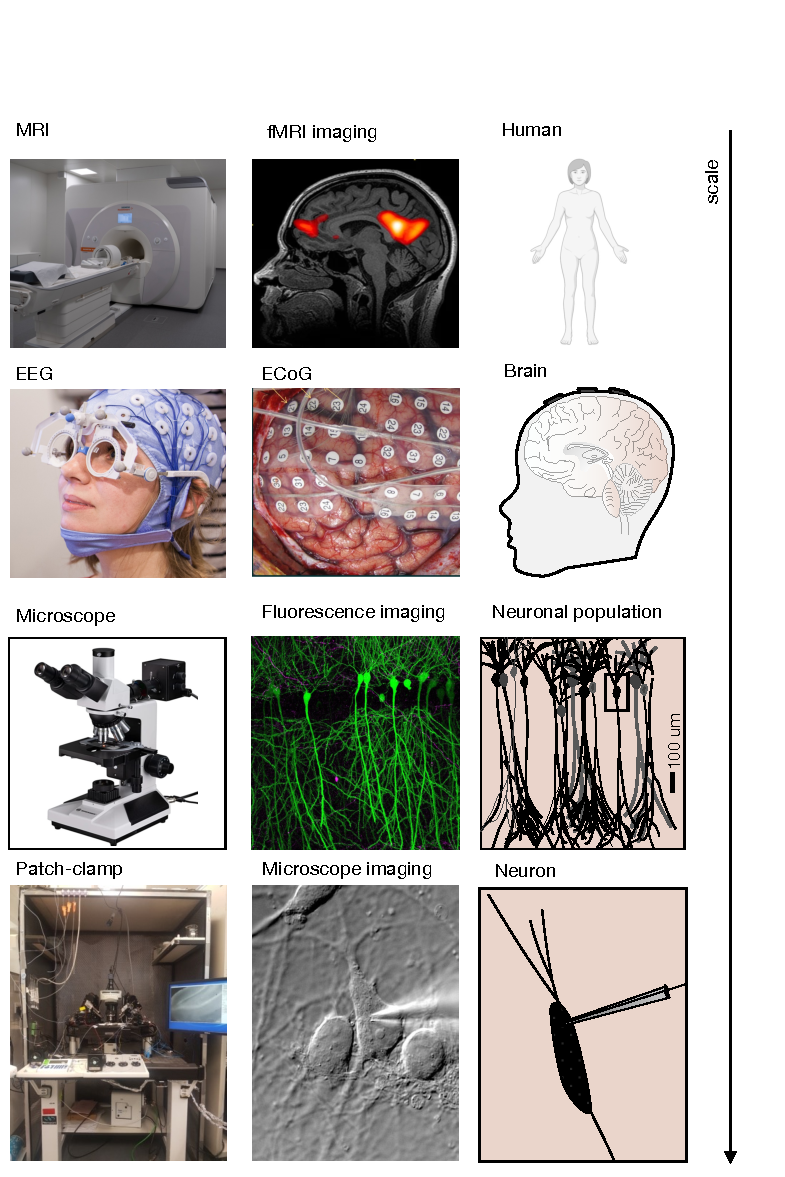
\includegraphics{latex/fig/Intro/Bgd_Tools.pdf}
    \caption{Caption}
    \label{fig:my_label}
\end{figure}



\begin{itemize}
    \item Behavior:\\
    Observing behavior is a simple and technically undemanding technique for gaining insights into human or animal functioning. It can yield valuable information about decision-making, memory retrieval, and sexual behavior among others. Researchers may passively observe behavior or request that participants perform specific tasks. 
    \item Brain imaging - using metabolic activity as indirect mesure of the neuronal activity
    \begin{itemize}
        \item[$\circ$] \acrfull{fMRI}:\\
        Neural activity induces change in metabolic processes such as blood flow or oxygen supply. This non-invasive technique indirectly measures brain activity in different brain regions by detecting variations in blood flow or oxygenation levels. The temporal resolution is not accurate enough to measure rapid changes in brain activity.         
        \item[$\circ$] \acrfull{PET}:\\
        Similar as fMRI, it is a non-invasive imaging technique using radioactive tracers to measuring metabolic activity such as blood flow or glucose uptake for example. 
    \end{itemize}
    \item \acrfull{EEG}:\\
    The EEG is a non-invasive technique using surface electrodes on the scalp. These electrodes record summed activity of large populations of neurons in large brain areas such as population activity of cortical neurons. It is commonly used to study brain rhythms which are associated with different cognitive states. 
    \item \acrfull{MEG}: \\
    MEG measures magnetic fields generated by the neural activity in the brain. Like EEG, it is a non-invasive technique that provides the overall activity of large populations of neurons. It is commonly used to record deeper structures such as thalamus and brainstem. 
    \item \acrfull{ECoG}: \\
    The ECoG is an invasive technique to record population activity of neurons in a large area (order of milimeters square) by placing a grid of electrodes directly at the surface of the brain. It recordes superficial layer of the brain.
    \item \acrfull{LFP}:\\
    Extracellular recording of a population activity of neurons in a localized area of the brain, typicalling using microelectrodes. It reflects the collective activity of populations. It is often used to study neuronal synchrony. 
    \item \acrfull{MEA}:\\
    Cluster of sensors recording up to hundred electrical activity of multiple neurons simultaneously.  
    \item Single neuron recording 
    \begin{itemize}
        \item[$\circ$] extracellular recording: by placing an electrode in the extracellular medium, this technique allows for the recording of sharp variations in the potential but not the membrane potential itself. It is useful for recording the neuronal rhythm. 
        \item[$\circ$] intracellular recording: a sharp pipette is inserted inside the neuron equipped with an electrical sensor to record the electrical activity of individual neurons.
        \item[$\circ$] patch-clamp: similarly as the intracellular recording, a glass pipette is used to create a seal between the pipette and the membrane. This allows the measurement of passing currents through the membrane with high precision. This technique provides a high temporal and spatial resolution but it is invasive and technically demanding. 
    \end{itemize}
    \item Microscope imaging:    \\
    To observe the anatomy of the brain, surgery, dissection and microscope provide inside about morphology of the different structures of the brain from organs to proteins. 
    \begin{itemize}
        \item[$\circ$] Optical imaging: by using a fluorescent substance, calcium concentration can be monitored during the brain or neuronal activity.
        \item[$\circ$]  Calcium Imaging: Calcium levels within the neuron indicating its activity can be recorded by measuring fluorescent dyes. 
        \item[$\circ$] Voltage-Sensitive Dye Imaging: Similarly to the calcium imaging, it uses fluorescent dyes to measure changes in the membrane potential of neurons.
        \item[$\circ$] Two-photon imaging: it is a type of microscopy to record neuronal activity by measuring fluorescent indicators. This device provides a good temporal resolution.  
        \item[$\circ$] Optogenetics: This technique permits to target and control the activity of particular cells by using light-sensitive proteins that are genetically engineering. 
    \end{itemize}

\end{itemize}
Each of these techniques has its own advantages and disadvantages with respect to their spatial or temporal resolutions and its invasiveness. Researchers must carefully choose the appropriate methods to answer their research questions. \\~\\
\smallbreak
\noindent
\begin{minipage}{0.45\textwidth}
\begin{lilashaded}
\textbf{\textit{In-vitro}, \textit{in-vivo} and i\textit{n-silico}}\\
~\\
These terms are sometimes confusing. Here is a brief reminder: \\
- \textit{in-vitro}, translated in glass: the experiments take place in a test-tube.\\
- \textit{in-vivo}, translated  in life: the experiments take place in the living organism. \\
- \textit{in-silico} refers to silicon chip used in computer: the experiments are performed on computers and via virtual simulations. 
\end{lilashaded}
\end{minipage}


\newpage
\begin{figure}[h!]
    \centering
    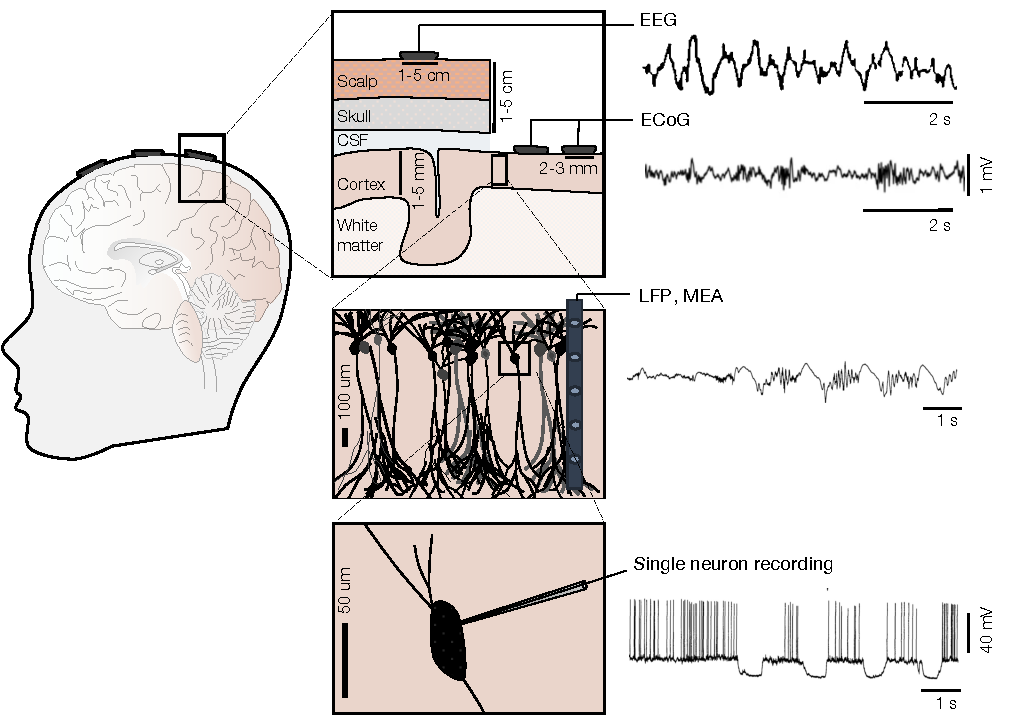
\includegraphics{latex/fig/Intro/Bgd_Recording.pdf}
    \caption{Caption  EEG \textcolor{red}{???}, ECoG \citep{konerding_2018} LFP, Single \citep{steriade_cellular_1995}}
    \label{fig:my_label}
\end{figure}
 



 
\newpage
% -----------------------------------
% -----------------------------------

%     BRAIN STATES
%
% -----------------------------------
% -----------------------------------
\section{Understanding brain states: from brain activity to neuronal activity}

% -----------------------------------
%       Brain state | at the brain level
% -----------------------------------
\subsection{Brain state identification}
Our everyday life is sequenced by different states. During the night, we sleep and dream,  and then we wake up and begin the day. We are capable of walking, looking around, and rapidly reacting to our environment . We can aslo engage in complex actions, think, and remember. These transitions between states are commanded by our brain \citep{bradley_state-dependent_2022}. 

A \textit{brain state} mirrors the overall activity pattern of neuronal population that can vary depending on the context. Indeed, the brain is made of interconnected neurons that communicate with each others, receive information and process it. Ongoing neural activities give rise to rich patterns that can be observed at different scales; from molecule and cell levels to microcircuits or networks up to the whole brain. Capturing brain states at a given spatial scale requires appropriate techniques: from neuronal recordings with pipette to population activity with LFP or EEG. The fluctuations between brain states occur at various timescales. At one extreme, brain states occur at hundreds of milliseconds during sharp shifts of attention, fast memory retrieval or when several action potential are generated in response to sensory stimuli, such as change in light intensity. Intermediatly, brain states are fluctuating in the range of hours with wake-sleep cycles. At the extreme case, brain states evolve over the course of brain development or during long-term changes in behavior, such as skill acquisition or recovery from injury. In the case of the slow progression into degenerative disease, the neural activity is no longer generating the correct brain state.

\begin{figure}[h!]
    \centering
    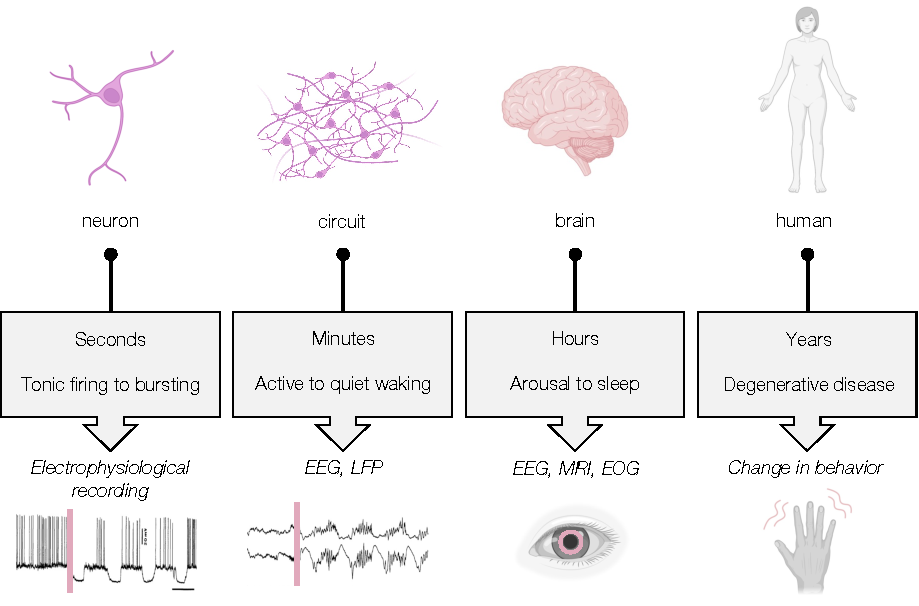
\includegraphics{latex/fig/Intro/Bdg_BScale.pdf}
    \caption{Caption}
    \label{fig:my_label}
\end{figure}

I follow the scientific definition provided in \citep{bradley_state-dependent_2022,zagha_edward_mccormick_neural_2014} telling that a brain state is "a recurring set of neural conditions that is stable for a behaviourally significant period of time. This set of neural conditions is often reflected in distinct patterns of ongoing activity but can also be revealed by neural responses to stimuli." 

Distinct brain states are characterized by distinct neural signatures mostly defined by the frequency and the spatiotemporal patterns of the LFP \citep{kringelbach_brain_2020}. They are often associated to identifiable cognitive or motor states. In addition, other features such as the breathing speed, the muscle tone, the eye movement, the pupil diameter, the heart beat might help to distinguish the brain states \citep{reimer_pupil_2014, mcginley_waking_2015}. 

\subsubsection{Classification and Characteristics of Brain Waves in Different States}
 There exists a large variety of brain waves that were classified based on the frequency content in the EEG or LFP oscillations \citep{tyree_optogenetic_2017}: 
\begin{itemize}
    \item gamma oscillations at 30 to 100Hz - associated with an engaged consciousness.  
    \item beta oscillations at 12 to 30Hz - associated with active waking, concentration and mental alertness.
    \item alpha oscillations at 8 to 12Hz - associated with quiet waking, resting, relaxed and calm state of mind.
    \item theta oscillations at 4 to 8Hz - associated with sleep, deep relaxation or meditation.
     \item delta oscillations at 0.5 to 4Hz - associated with deep sleep, the slowest brain waves.
    
\end{itemize}

\begin{wrapfigure}{r}{0.5\textwidth}
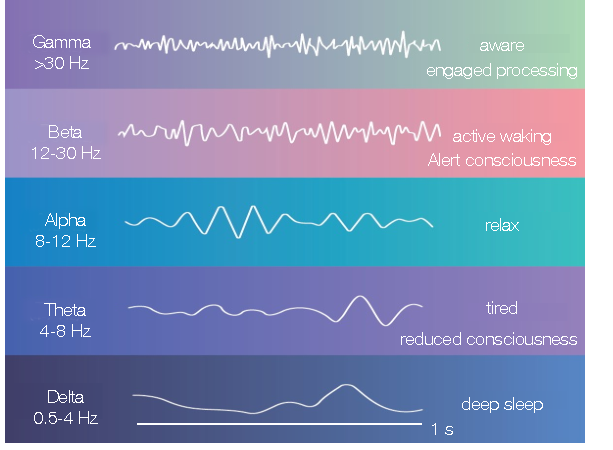
\includegraphics[scale=0.75]{latex/fig/Intro/Bdg_BrainWaves.pdf}
\caption{...}
\label{fig:BrainWaves}
\end{wrapfigure}

The familiar example of sleep helps to get more insight about the fluctuations in brain states \citep{mcginley_waking_2015, molnar_cell_2021} Classically, deep sleep is characterized by a large-amplitude and low-frequency signal with no eye movement and reduced muscle tone, referred as \acrfull{NREM}, associated with a succession of delta and theta oscillations). By opposition, waking is associated to small-amplitude faster frequency fluctuations (associated to a mixture of alpha and beta oscillations). These two stages are often described respectively as a global synchronization dominated by low frequency content or global desynchronization.  The term \acrfull{REM} is often encountered for the dream stage that looks similar as the waking state except paralyzed muscle tone and rapid-eye-movement are observed. 

This simplistic distinction between waking and sleep have been challenged and the concept of active and quiet waking have been introduced. During waking, larger-amplitude, lower-frequency oscillations are observed for example in the somatosensory, visual, and auditory cortical regions. They are associated to quiet waking. These oscillations are suppressed as soon as human or animals enter active waking due to for example motion or attention shift \citep{mcginley_waking_2015}. 


\subsubsection{Fluctuations in brain states}
The brain's evolution during a given action or mindset is a fascinating phenomenon, as is understanding how the transition between different states occurs. For instance, when we are meeting someone important, our heart rate increases, our hands sweat, and our body temperature rises, all of which are orchestrated by the brain operating in an alert state. Various pathways, such as brain circuitry, movement-related factors, and breathing, influence the transition between states \citep{tantirigama_perspective_2020}. However, neuromodulation is the major factor that affects the transition. Figure \textcolor{red}{XXX} provides insight into the close relationship between brain states and neuromodulators. The cocktail of chemical substances is constantly fluctuating. During active waking, the brain has a high concentration of acetylcholine, noradrenaline, serotonin, dopamine, and histamine. These concentrations decrease in quiet waking and are very low during \acrfull{NREM} sleep.

Several diseases, such as schizophrenia, epilepsy, autism, Alzheimer's, and Parkinson's disease, dramatically alter brain states \citep{uhlhaas_neural_2006, kuhn_event-related_2004, cannon_neurosystems_2014}. Parkinson's disease, for instance, is often recognized by motor dysfunctions such as arm tremors, which is explained by a drastic change in the expected brain state. \textcolor{red}{add image of brain state switches with the figure}

The mechanisms underlying switching between brain states are not yet fully understood. Studying the interplay between neuromodulation and switches in brain states at the cellular level can provide insight into these mechanisms.




\begin{figure}[h!]
\hspace{-1cm}
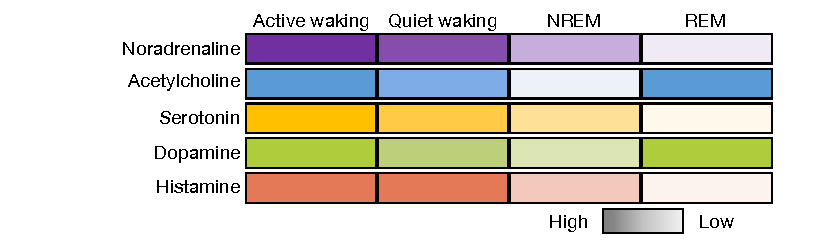
\includegraphics[scale=1]{latex/fig/Intro/Bgd_NMODinBS.pdf}
\caption{ .... 
Inspired by \citep{tyree_optogenetic_2017} }
\label{fig:intro_tyree_opto}
\end{figure}

 

% -----------------------------------
%       Brain states: at the neuron level
% -----------------------------------

\subsection{Neuronal activity reflects the brain state}

The diversity of neurons in the brain is what allows for the myriad of brain states that we experience. Neurons come in different morphology, shapes and sizes, and possess unique types of ion channels which allow them to generate electrical signals and communicate with other neurons. Their different neuronal properties allow them to generate firing pattern. \textit{Firing pattern} refers to the way the neuron produce an action potential over time.  It depends on the neuron itself as well as the timing and the intensity of the received stimulus. The term neuronal excitability is often encountered in literature and refers to the ability of a neuron to generate an action potential in response to a stimulus.



\subsubsection{Classification of neuronal firing patterns}
Figure \textcolor{red}{XXX - tous les firing patterns} uncovers the existence of the different firing patterns often encountered. This is a non-exhaustive list and description of these patterns \citep{komendantov_quantitative_2019, izhikevich_classification_2004}:
\begin{itemize}
    \item \textit{tonic firing}: the neuron produces a succession of action potentials in response to an external stimulus or a sustained input (also called tonic spiking, regular spiking).
    \item \textit{bursting}: the neuron generates a sequence of clustered action potential occuring at high frequency separated by silent periods \citep{kucyi_neural_2017}.
    \item \textit{pacemaking}: the neuron generates a constant succession of action potentials at a fixed frequency independently of any external input, only by relying on its intrinsic properties.
    \item \textit{adapting spiking}: the generates a succession of action potentials with a gradual decrease in their firing rate over time in response to a constant stimulus.
    \item \textit{plateau potential}: the neuron can maintain its spiking activity for a relatively long period of time after the occurence of an excitatory stimulation, it is a form of bistability \citep{marder_plateau_2003}.
    \item \textit{rebound burst}: burst of action potentials in response to an hyperpolarization input.\\
\end{itemize} 

The Blue Brain project engages in a gargantuan challenge: the reconstruction and simulation of a column of the neocortex. They model different cell types classified based on their morphology and their firing patterns  \citep{markram_reconstruction_2015}.  I decided to focus my interest in two firing patterns: tonic spiking and bursting. 


\begin{figure}[h!]
    \centering
    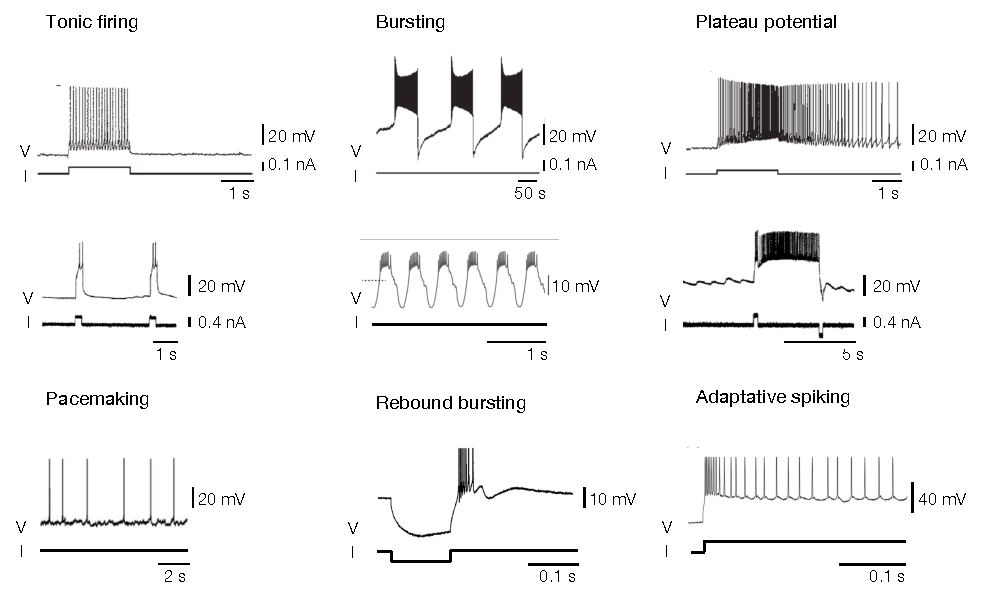
\includegraphics{latex/fig/Intro/Bgd_FiringPattern.pdf}
    \caption{Tonic (dorsal \citep{marder_plateau_2003}, DG \citep{weimann_effects_1993}), Burst (dorsal \citep{marder_plateau_2003}, lateral pyloric \citep{marder_from_2021}),  Pacemaking (\citep{ramirez_role_2011}, Plateau (dorsal \citep{marder_plateau_2003}, DG \citep{weimann_effects_1993}  }
    \label{fig:my_label}
\end{figure}

\begin{comment}
\begin{figure}
    \centering
    \includegraphics{fig/Intro/Izhikevich_classification}
    \caption{"Summary of the neuro-computational properties of biological spiking neurons [Izhikevich, 2004]. This figure is re- produced with permission from www.izhikevich.com. (Electronic version of the figure and reproduction permissions are freely available at www.izhikevich.com)." \citep{izhikevich_classification_2004}}
    \label{fig:intro_izhikevich}
\end{figure}
\end{comment}

\subsubsection{Bursting: Definition, Characteristics, Shape, and Mechanisms of generation}
Already investigated 25 years ago, this firing pattern was defined by "clusters that often last at most \SI{25}{ms} and contain several action potentials from two to 6 at a high frequency (about \SI{200}{Hz})" \citep{lisman_bursts_1997}. The interest for this particular firing pattern has continued to grow. 
~\\
\textit{Brain regions containing neurons able to burst}\\
Bursting is observed in several brain regions  \citep{shao_neural_2021, zeldenrust_neural_2018} such as in the cortex, mostly in pyramidal neurons, in the hippocampus, in the pyramidal neurons in CA1 region, the thalamus, in the thalamocortical and neurons of the reticular nucleus, in the hypothalamus, in gonadotropin-releasing hormone (GnRH)  neurons, in the cerebellum, in purkinje and granules cells,  in the brainstem, in the ventral tegmental area, in dopaminergic neurons. It is also observed outside the brain and in different species such as in pre-Botzinger complex - in the respiratory neurons, in stomatogastric ganglion in crustaceans - in anterior bursting neuron, in abdominal ganglion in aplysia - in neuron R15,  in circuit involved in central pattern generator \citep{grillner_CPGs_2021}, in pancreatic beta cells \citep{jeong_bursting_2012}. 

~\\
\textit{Bursting are characterized by several features}\\
Bursting can be described by different features \citep{van_pottelbergh_robust_2018, drion_novel_2012} 
\begin{itemize}
    \item The \textit{active period} is the duration composed of the succession of action potentials, called the burst or spike train. 
    \item The \textit{quiescent period} is the silent period between the spiking period, also called intraburst interval.
    \item the \textit{intraburst period} is the timing between two distinct burst of action potential. 
    \item the \textit{intraburst frequency} is the inverse of the intraburst period. 
    \item the \textit{interburst period} is the timing between two action potentials inside the burst, also called inter-spike interval. It can vary within the burst. 
    \item the \textit{interburst frequency} is the inverse of the interburst period. 
    \item the \textit{duty cycle} is the ratio between the intraburst period and the interburst period. 
    \item the number of \textit{\acrfull{SPB}}.
    \item the \textit{spike latency} is the delay between the start of the depolarization and the start of the spike train.
    \item the \textit{plateau} potential: the burst of action potentials occur at a more depolarized potential than the hyperpolarized state. It allows to identify an up and down state in the firing pattern. 
    \item the \textit{\acrfull{ADP}} the burst is finished by a small depolarization bump before hyperpolarizing.
\end{itemize}



~\\
\textit{Bursting can take several shapes}\\
Bursting can display different signatures that are described by the oscillations \citep{desroches_classification_2022, drion_novel_2012, van_pottelbergh_robust_2018, smith_fourier_2000}: 
\begin{itemize}
    \item  the \textit{parabolic bursting}: the train of spikes is at a noticeable depolarized state with respect to the hyperpolarized membrane voltage. It is observed in Aplysia R15 for example \citep{adams_slow_1985, turrigiano_selective_1995}
    \item the \textit{square wave bursting}: the neuron discharges continuslouly during the active period and stop without a noticeable plateau potential. It is observed in pancreatic beta-cells \citep{bertram_phantom_2008} but it is more often encountered in mathematical models. 
    \item the \textit{elliptic bursting}: the burst is a bit more depolarized compared to the parabolic bursting observed in sensory neurons.
    \item the \textit{pseudo-plateau bursting}: a strong plateau potential is observed and the amplitude of the successive action potentials in decreasing. 
\end{itemize}

~\\
\textit{Mechanisms behind bursting}\\
Two categories of burst generation are considered according to \citep{jeong_bursting_2012,jeong_bursting_2012} : 
\begin{itemize}
    \item forced burst generation: the burst is the consequence of stimulation with a current that drives the neuron above or below the action potential threshold. This current can be the result of either an external simulation via an electrode - for example a square-wave signal current or synaptic input. In the case of synaptic input, either the neuron is normally spiking but a periodic inhibitory provokes intervals of silence or the neuron is silent and receives periodic excitatory synaptic input causing the clusters of action potentials (see Figure \ref{fig:intro_burst}) 
    \item intrinsic burst generation: the neuron is able to burst due to the different ion channels. Their opening and closing kinetics orchestrate the intrinsic generation of bursting such that intrinsic currents depolarizes the neuron until it reaches its firing threshold, allowing the occurrence of several action potentials. Then, the neuron hyperpolarizes on a ultraslow timescales. This sequence is repeated due to the interaction of the different ion channels. Experimental neuroscientists have been trying to identify the ionic currents necessary in this autonomous pattern generation. The T-type calcium channels have been recognized to play an important role \citep{cain_contributions_2010} (see Figure \ref{fig:intro_burst}) . 
\end{itemize}



\begin{figure}[h!]
    \centering
    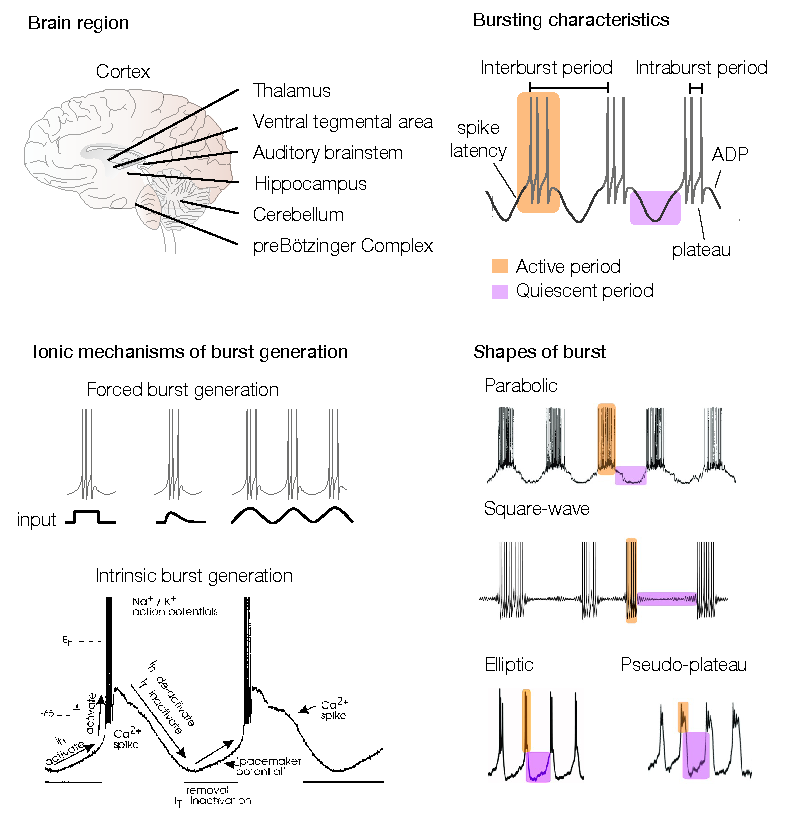
\includegraphics[scale=1]{latex/fig/Intro/Bgd_Burst.pdf}
    \caption{\citep{zeldenrust_neural_2018, desroches_classification_2022, mccormick_sleep_1997}}
    \label{fig:intro_burst}
\end{figure}

~\\
\newpage
\subsubsection{Neurons are able to switch between firing patterns}
Neurons are fundamental units of the brain; their variety in morphology, roles and now their firing patterns is at the basis of the complexity and power of our  brain.  Figure \textcolor{red}{XXXX} shows that firing pattern vary from one neuronal population to the other. But most surprisingly, one neuron can switch from firing pattern to an other firing pattern. It is mainly caused by the modulation of ion channel properties. Several factors can modulate these properties such as:
\begin{itemize}
    \item neuromodulation (like dopamine, serotonin or acetylcholine): neuromodulators alter the ion channels for example by blocking or recruiting them, changing their densities, altering their kinetics \citep{steriade_novel_1993}. 
    \item synaptic input: a inhibitory input can switch a neuron from regular spiking to bursting by activating some ion channels that were previously closed. 
    \item environmental changes: temperature and pH among others are external factors that can modify the ion channels \citep{hedrick_effect_2012} (see Figure \ref{fig:intro_switch} XXXX)   
    \item other mechanisms such as change in the resting potentiel or changes in the extracellular concentration of potassium \citep{frohlich_coexistence_2006}.
\end{itemize}


\subsubsection{Switches from tonic spiking to bursting}
\textit{Mechanisms at the cellular level}\\
The thalamic neuron has been a nice support since many years to understand what are the key mechanisms between the transition from tonic spiking to bursting \citep{mccormick_sleep_1997, cain_contributions_2010} (see Figure \ref{fig:intro_switch}\textcolor{red}{XXX}).  This neuron is mainly driven by sodium current, potassium current, T-type calcium current and hyperpolarization-activated current (H current). At a depolarized state, the neuron is governed by the dynamics of the sodium and potassium channels generating succession of action potentials. Due to change in the neuromodulatory state for example, the neuron is hyperpolarized that results in calcium channels. They open in a slow timescale generating a calcium influx that depolarizes the neuron (see Figure \textcolor{red}{XXXX}). Sodium and potassium current interplay to produce action potentials. Simultaneously, calcium channels close on a ultraslow timescale. The neuron hyperpolarizes, no more action potential is generated. The hyperpolarization-activated current enters into account to depolarize the neuron and activate the whole process again. 

To switch from tonic spiking to burst, the neuron must be hyperpolarized to allow the activation of calcium channels. As explained earlier in the mechanisms of switches, this can be achieved by applying an external hyperpolarized current or neuromodulators affect the ion channel properties and set the neuron in a hyperpolarized state. \\
~\\
~\\
\textit{Switching from tonic spiking to bursting is not only associated to transitions from wakefulness to sleep}\\
The switch from tonic spiking to bursting is drastically impacting the brain states as earlier explained that neuronal activity is shaping these states \citep{takahashi_neuronal_2006}. This section is explaining the relationship between this switch at the cellular level into the switch in brain state and the associated behavioral state. 

The switch from tonic spiking to bursting is often associated to the transition from wakefulness to sleep. Indeed, during wakefulness, neurons are reacting to incoming signals and discharges accordingly in tonic spiking. This is translated at the population level by a small, high-frequency signal. Transitioning to sleep, neurons are bursting, a synchronization of the activity is created resulting in a large, low-frequency LFP signal \citep{mccormick_sleep_1997}. It is often encountered to talk about active (up) and inactive (down) periods occurring at low frequency. Tonic mode was thought to be the default mode during wakefulness to relay the information while bursting mode was associated to a blocking of the information from the external mode. 

But more and more evidence confirms that bursting occurs during wakefulness \citep{fanselow_thalamic_2001, steriade_natural_2001, zagha_edward_mccormick_neural_2014, reimer_pupil_2014}. Some recordings were even obtained in monkey \citep{guillery_thalamic_2002} while in the past it was mainly on rodents and cats. Bursting plays a role in the information processing during waking behavior \citep{sherman_tonic_2001,ramcharan_burst_2000}. This is explained by the presence of slow oscillatory activity during quiet waking with absence of movement. As soon as the animal walks, the slow rhythmic activity is suppressed \citep{mccormick_brain_2015}. "While the slow oscillation was once thought to be restricted to periods of slow wave sleep, animal studies now suggest that it may occur in the waking state, particularly during periods of inattentiveness or drowsiness"
 
These switches in wakefulness have an impact on sensory processing \citep{steriade_natural_2001}. This bidirectional switch allows to meet changing behavioral demands \citep{crandall_corticothalamic_2015}. 

~\\
\textit{Examples from Dopaminergic Neurons, Sensory Processing, and Neurological Diseases}\\
This section provides several examples of switches from tonic firing to bursting and their corresponding switches in brain states and behavior. 

Dopaminergic neurons have three modes of discharge: pacemaking, phasic or bursting \citep{tsai_phasic_2009, johnson_burst_1992}. Without stimulation, the neuron is in pacemaking mode. It fires at a small frequency around \SI{1}{Hz}. During a stimulation, the frequency increases during the applied input. Finally, under special conditions, neurons is bursting. The switch from regular spiking to bursting is observed in paradoxal slep and palatable food consumption \citep{dahan_prominent_2007, ji_tuning_2009}. 

Neurons in the cortex are sensitive to drugs like ketamine. \citep{cichon_ketamine_2023} observed that drugs can trigger 'non-ordinary brain states' by suppressing the spontaneous activity of some neurons and activating some silent ones. The brain enters a particular mode in which it is disconnected of the external environment but still performing internal subjective experiences \citep{cichon_ketamine_2023, yang_ketamine_2018}. 

We have the ability to switch from hearing to listening. It is translated by a switch in brain states mirroring the switch in neuronal activity in the auditory cortex and other brain regions \citep{de_franceschi_task-induced_2021}. It is confirming that sensory inputs in this case sound is processed in different manners depending on the neuronal firing patterns. This state-dependent sensory processing also occurs in the olfactory cortex \citep{murakami_state-dependent_2005}. Response to smells is bigger while neurons are spiking compared to the weaker response while neurons are in low-frequency rhythm. 


Some diseases are marked with pathological brain states. As mentioned earlier, parkinson or alzheimer diseases are well-known examples of abnormal brain oscillations compared to normal conditions. In normal conditions, neurons in the subthalamic nucleus (STN) neurons and globus pallidus (GP) neurons are in tonic activity - characterized by an small amplitude, high frequency content at the population level. In abnormal conditions (in PD), the STN and GP are in low-frequency rhythmic bursting \citep{bevan_move_2002, beurrier_subthalamic_1999}. In the context of dystonia - a neurological disease that causes the muscles to contract involuntarily, purkinje cells that were tonically spiking in control conditions exhibit a abnormal high-frequency bursting \citep{fremont_abnormal_2014}. For pain processing, depending on the operation mode of the neuron: the pain is differently processed by our brain. In spiking mode, the innocuous stimuli are associated to acute nociception, while the generation of plateau potentials, by increasing the excitability of deep dorsal horn neurons plays a role in central sensitization \citep{marder_plateau_2003}. To illustrate with a simple example, the contact with a needle can be interpreted by three sensations: either pain is only felt when the needle touches the skin (spiking mode), or pain persists after the needle removal (plateau potential mode) or pain is abnormally felt even without simumus (bursting mode). There are also examples in the context of anxiety, depression epilepsy, schizophrenia, addiction among others. Better understanding the modification of discharge patterns could help to develop therapeutic treatments. 



\begin{figure}
    \centering
    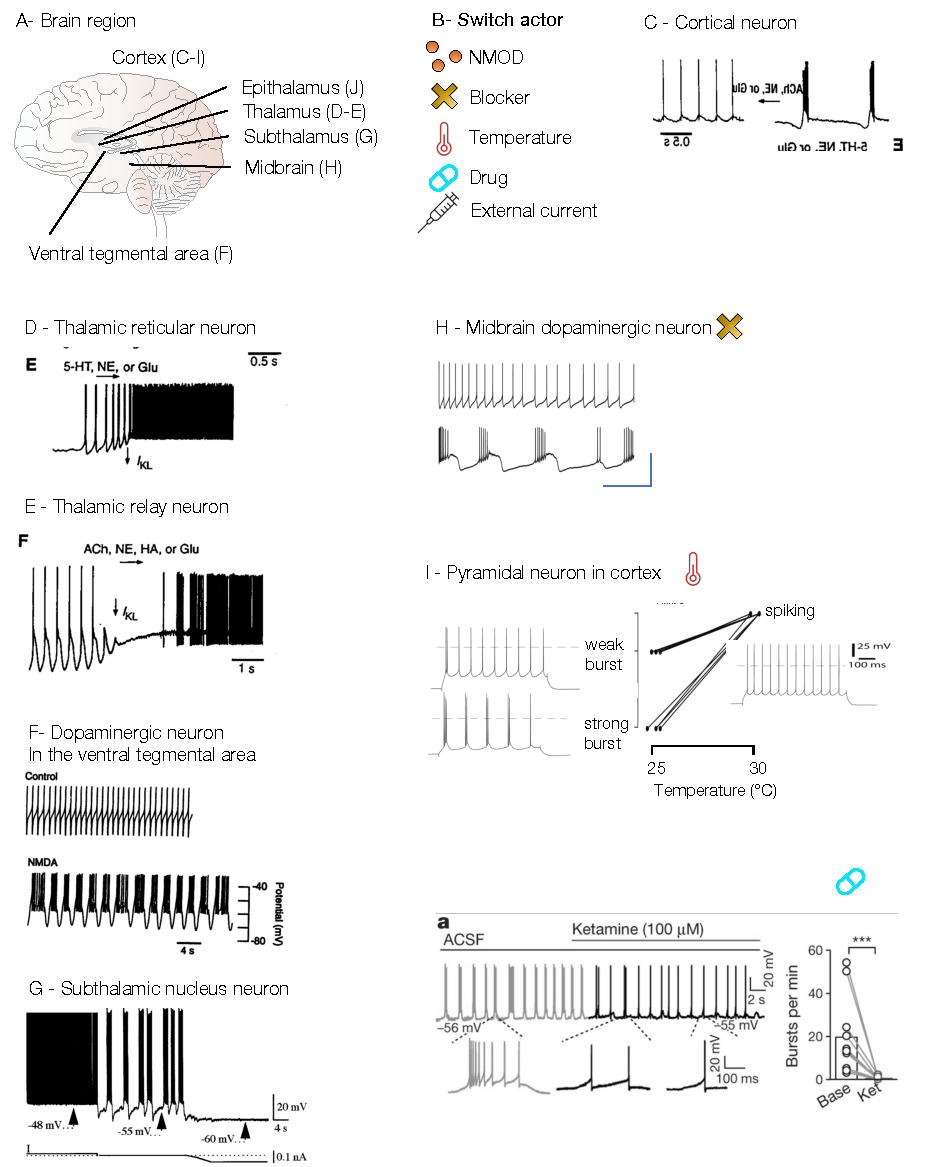
\includegraphics{latex/fig/Intro/Bgd_Switch.pdf}
    \caption{\citep{mccormick_sleep_1997, ji_tuning_2009, johnson_burst_1992, hedrick_effect_2012} McCormick (anesthesized cat), Ji (rats), Jonhson (), T (mice), Cichon (rodent ket), Yang (rodent ket- artificial cerebrospinal fluid , Locomotion (Polack), Wake-sleep (Steriade 2001)) \textcolor{red}{retravailler l'ordre de l'image: montrer les deux neurons thamalamiques en mettant aussi le behavior puis montrer des switches dans le cortex eveil sommeil/locomotion puis DA neurons puis Temperature et drug)}}
    \label{fig:intro_switch}
\end{figure}

Yang: "but completely eliminated spontaneous burst firing within seconds of application"
\begin{comment} --- le texte est bien formulé ---
"Neural oscillations are a hallmark of cortical network dynamics (Buzsaki and Draguhn, 2004). Sustained oscillatory activity can be broadly classified as either tonic firing or bursting. Neurons in a number of brain structures including the thalamus (Jahnsen and Llinas, 1984a,b) and neocortex (McCormick et al., 1985; Connors and Gutnick, 1990) exhibit either tonic firing or bursting in a state-dependent way. One of the most dramatic examples of global transitions between bursting and tonic spiking regimens is the transition from slow-wave sleep to rapid eye movement sleep or waking in the thalamocortical system (Steriade et al., 1993, 2001; Timofeev et al., 2001; Steriade and McCarley, 2005). Slow transitions between a slow-wave state and a fast-wave state were also observed in the olfactory cortex (Murakami et al., 2005). Coexistence of bursting and tonic spiking regimens is not limited to vertebrates (Lechner et al., 1996; Turrigiano et al., 1996; Shilnikov et al., 2005). Different levels of synaptic excitatory drive, activation of intrinsic conductances by neuromodulation, and changes in the extracellular ionic environment control the state-dependent oscillatory regimen" --- >MODEL (bazhenov)\\
\end{comment}


\newpage
\section{Neuromodulation: link between switches in neuronal activity, brain states ...}
\textcolor{red}{Décider si on met la neuromodulation ici ou au dessus}


\begin{pinkshaded}
Neuromodulators are powerful substances in our brain that control and allow us to rapidly react. Their mechanisms are complex due to their diffuse projecting and their broad operating modes. Figure~\ref{fig:Bgd_NMOD} confirms that studying the effects of neuromodulators is a real struggle due to their multiple targets and their coordinated actions. 

Aa smart strategy to investigate neuromodulation is to move to small circuit as done in the impressive work of Eve Marder. Crustaceans have well-defined neuron circuits and are multiply modulated \citep{marder_understanding_2007}.

Neuromodulators affect the neuron circuit by changing the frequency, the number of spikes per burst so that a same circuit can display several output patterns. The mechanisms underlying these changes have investigated in the last 30 years \citep{nadim_neuromodulation_2014, marder_understanding_2007}: 
\begin{itemize}
    \item One neuromodulator may affects different voltage-gated ion channels.
    \item Individual neuromodulators may have different actions on a neuron by altering different physiological mechanisms .
    \item Different neuromodulators may have a converging action on a same voltage-gated ion channels.
    \item Neurons and synapses are affected by neuromodulators. 
\end{itemize}

(...) It rises the question of how is it possible to alter as many parameters and simultaneously maintain a network output. 

~\\
----\\
back to the future\\

Then the effects of descending modulatory projection neurons on the STG are removed by either cutting or blocking the input nerve to the STG, the fast pyloric rhythm either stops completely or slows down (Figure 3, control). Under these conditions, exogenous application of a large number of different substances can elicit a triphasic motor pattern


effect of DA: \\
An unexpected result from this work is that dopamine modulates several currents in the same neuron and that the same current can be modulated differently in different target neurons


Understanding how circuits can be stable in the face of ubiquitous neuromodulation is an important and deep problem.
stability mechanisms 1) si un NMOD jour sur un courant inward et outward, le resultat va etre le meme. 


Can Modulator Action Be Robust and Predictable Despite Variability in Underlying Conductances? Much computational and experimental evidence shows that there can be considerably variability across animals or across neurons in the parameters that control neuronal excitability and network function even when the circuit output is maintained

\end{pinkshaded}



\begin{figure}[h!]
    \centering
    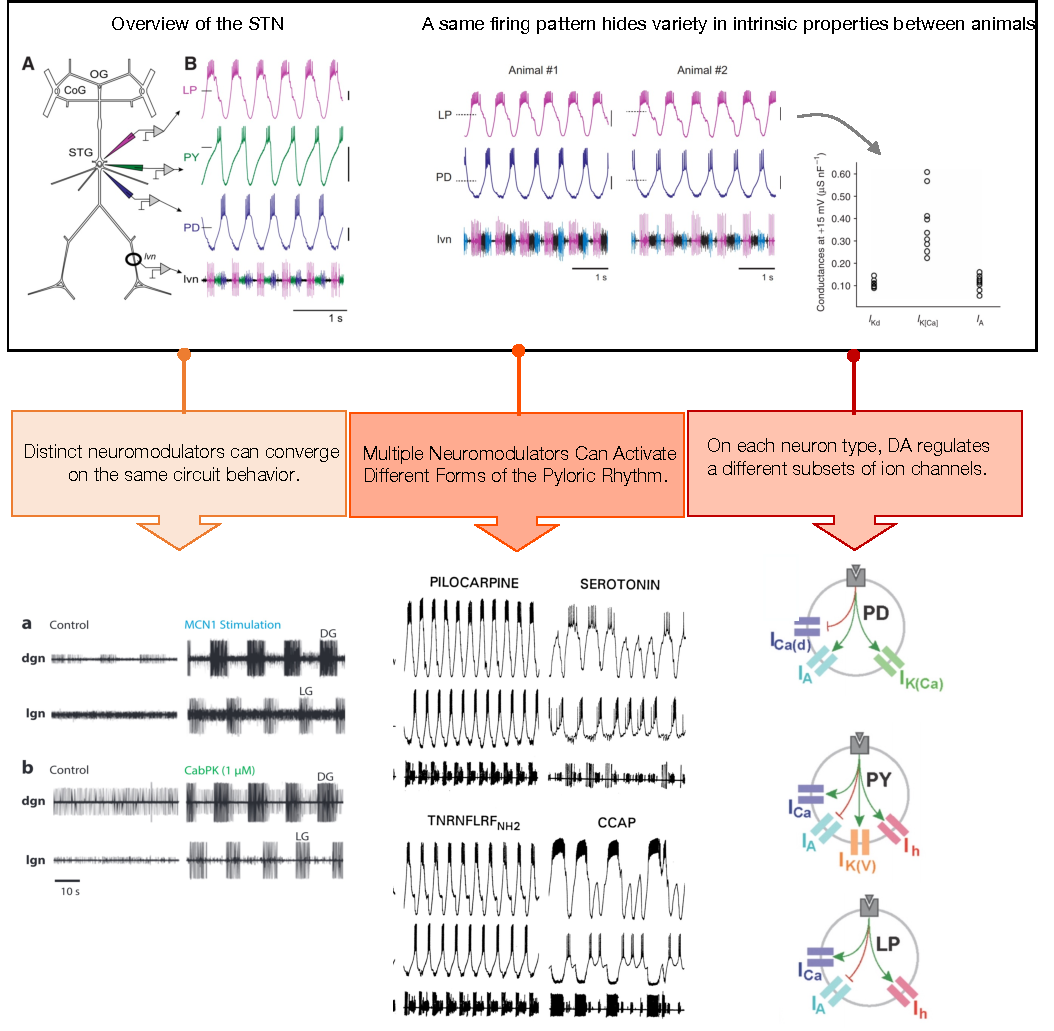
\includegraphics{latex/fig/Intro/Bgd_Marder.pdf}
    \caption{Diagram \citep{marder_neuroscience_2021}, conductance distribution \citep{schulz_variable_2006}, (bottom-left)  \citep{marder_neuromodulation_2014} (bottom-middle) \citep{marder_neuromodulation_2012}  (bottom right) \citep{marder_understanding_2007}}
    \label{fig:my_label}
\end{figure}

\newpage
~\\
\newpage
% -------------------------
% -------------------------
%
%     SYNAPTIC PLASTICITY
%
% -------------------------
% -------------------------
\section{Synaptic plasticity}

\begin{comment}
Our neurons have the ability to modify their connections with each other, a property called \textit{synaptic plasticity}. 
According to \citep{citri_synaptic_2008}, it refers "to the activity-dependent modification of the \textit{strength} or \textit{efficacy} of synaptic transmission" at synapses \citep{citri_synaptic_2008}. 

Before digging further into the concept of synaptic plasticity, it appears mandatory to introduce the different concepts of  synaptic transmission, synaptic strength or synaptic efficacy among others.
\end{comment}
\textcolor{red}{INTRO}

\subsection{Synapse: definition, structure and functioning}
The term \textit{synapse} originates from Greek sunapsis, from 'sun' that means together and 'hapsis' that means joining from the verb 'haptein', in total it gives joining together. It corresponds to the junction where information is transmitted. It consists of the presynaptic terminal (the end of an axon), the gap between the two neurons (synaptic cleft) and the postsynaptic neurons that contains receptors (dendritic spine). 


The \textit{synaptic transmission} corresponds to the ability of neurons to transmit the information between each other. An action potential generated at the presynaptic neurons reaches the axon terminal and it is converted into a chemical signal that corresponds to neurotransmitter release. These neurotransmitters bind to the postsynaptic neurons that generate a response. The \textit{synaptic strength} refers to the magnitude of this synaptic response that can be recorded as an \acrfull{EPSP} or \acrfull{EPSC} (for excitatory synapse).  In the literature, the terms synaptic strength and synaptic efficiency are interchangeable, while the synaptic strength reflects the response magnitude, the  \textit{synaptic efficiency} defines how well a synapse transmits information. 

The synaptic strength can be increased or decreased and it is what makes our brain plastic and able to adapt the connections between neurons. Before exploring all the plasticity mechanisms, a more accurate description of the synaptic transmission and the synapse is required.







\subsubsection{Synaptic transmission}
The information transmission consists in three main steps as shown in Figure \ref{fig:SP_SynTrans}: (i) the action potential at the presynaptic neuron is triggered  glutamate release, (ii) glutamate binds to the postsynaptic receptors, (iii) the postsynaptic receptors allow flow of ions inside the postsynaptic neurons that generate a change in the postsynaptic membrane voltage.\\
~\\
\begin{wrapfigure}{l}{0.4\textwidth}
 \centering
    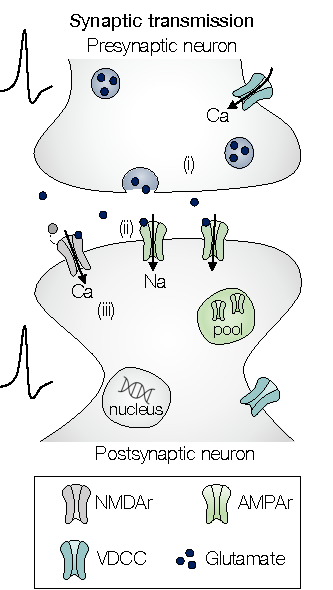
\includegraphics[scale=0.8]{latex/fig/Intro/SP_SynTrans.pdf}
    \caption{caption}
    \label{fig:SP_SynTrans}
\end{wrapfigure}
(i) The membrane depolarization at the presynaptic neuron terminal allows calcium to cross the membrane which trigger a signalling cascade. Synaptic vesicles containing neurotransmitters fuse with the membrane and release the stored neurotransmitters in the synaptic cleft 

~\\
(ii) Glutamate bind to two postsynaptic receptors that perform distinct roles in both synaptic  transmission and synaptic plasticity.  The first of these receptors is \acrshort{AMPAr}, an ionotropic receptor that opens when glutamate binds to it. Once activated, sodium and potassium ions primarily flow through the membrane, resulting in a increase in the postsynaptic membrane voltage. The second type of receptors is the \acrshort{NMDAr}, which is a metabotropic receptor that opens under two conditions, namely when glutamate binds to it and the magnesium blockage is removed. This removal of the blocker enables ion flow through the channel when the membrane voltage is sufficiently depolarized. This receptor are primarily selective for calcium ions, but also allow sodium and potassium ion flow. 

~\\
(iii) Both \acrshort{AMPAr} and \acrshort{NMDAr} work together to mediate synaptic transmission. Glutamate released from the presynaptic neuron binds to both receptors, but only opens the \acrshort{AMPAr}, resulting in ion flow and membrane depolarization. This depolarization triggers the removal of magnesium blocker, allowing \acrshort{NMDAr} to open, as the two activation conditions are fulfilled. The \acrshort{NMDAr} are often called coincidence detector as its activation requires a presynaptic activity causing glutamate release and a postsynaptic activity causing depolarization to remove Mg2+ block. Calcium flows into the postsynaptic neurons.



As I will add more details below, calcium plays a crucial role in the process of synaptic plasticity and it is why it is really important to understand how and why it enters the postsynaptic neuron.  Another source of calcium entering the postsynaptic neurons is voltage-dependent calcium channels such as L-type or T-type among others \citep{lamprecht_structural_2004}. These calcium channels can amplify the depolarization. 

Finally, the postsynaptic neuron responses to the presynaptic neuron action potential. It can be measured by the \acrfull{EPSP} or \acrfull{EPSC} \citep{citri_synaptic_2008}.


\subsubsection{Details on the spine composition}
As just described, postsynaptic receptors are principal actors in the synaptic transmission. They are located at a particular region of the postsynaptic neurons: on the \textit{spine}. 

The dendritic spine is a small protrusion at the surface of the dendrite that receives the input from other neurons (see Figure \ref{fig:SP_spine}A). It consists in a thin neck and a spine head. The dendritic spines contains receptors, channels, signalling molecules, which are useful for its functional role and protein scaffolds, which provide the spine structure \citep{bozelos_impact_2017}. These receptors, basically \acrshort{AMPAr} and \acrshort{NMDAr}, are concentrated at the tip of the spine in a visually distinct site called the \acrfull{PSD} \citep{bonilla-quintana_can_2022}.

The spine morphology is characterized by several geometric features: the length and the width of the neck, the volume of the head, the surface area of the \acrshort{PSD}. These features are correlated with the number of postsynaptic receptors as well as the readibility of transmitter pool, resulting in the efficacy of the synaptic transmission  \citep{Borczyk_neuronal_2019}.

Based on these features, spines can be classified into three categories (see Figure \ref{fig:SP_spine}B): (1) filopedia is a finger-like spine, (2) thin spine, (3) mushroom spine and (4) stubby spine. Logically, spines with a larger head and a larger propose a stronger connection between the pre- and the postsynaptic neurons \citep{bonilla-quintana_can_2022, lamprecht_structural_2004}. The spin shape relies on the spine cytoskeleton, composed with \textit{actin} filaments.  

The spine has the ability to compartmentalize calcium influx that empowers it with a input-specific property. \\

\begin{figure}[h!]
    \centering
    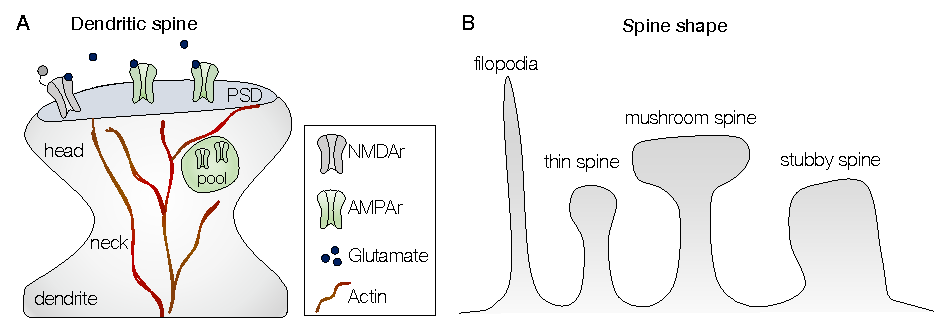
\includegraphics[scale=0.9]{latex/fig/Intro/SP_Spine.pdf}
    \caption{Caption}
    \label{fig:SP_spine}
\end{figure}



\subsection{Plasticity: from early to late change }
How do neurons adapt their synaptic strengths with each other or in other words, how do synaptic plasticity work ?  This is Scientists are  \citep{takeuchi_synaptic_2014}. Ramon y Cajal proposed theoretical hypotheses about the change in synaptic transmission in the mid-twentieth century \citep{cajal_estructura_1888}. Followed by Donald Hebb that brought attention about plasticity with his famous quote "cells that fire together, wire together" \citep{hebb_organization_1949}. Experiences on Aplysia provide some of the first evidence that synaptic strength change in response to stimuli \citep{kandel_behavioral_1979}. In parallel, \citep{bliss_long-lasting_1973} who introduced the notion of \acrfull{LTP} and \acrfull{LTD}, a a form of long lasting synaptic plasticity. \acrshort{LTP} involves a persistent increase of synaptic strength, while \acrshort{LTD} involves a persistent decrease of synaptic change \citep{lamprecht_structural_2004}. 

Nowadays, researches on synaptic plasticity is exploding; from understanding the molecular mechanisms to the formation of new networks. It confirms that synaptic plasticity can be described by many forms and mechanisms and that is also region-dependent. It can span from miliseconds to hours, days and even longer \citep{citri_synaptic_2008}. I will first recall what are the different quantitative measures of plasticity, the different tools used to record plasticity and what are the most encountered plasticity-induced protocols. Then, I will enter the core of the plasticity mechanisms from short-term plasticity to longer-lasting synaptic changes.  

%\textcolor{gray}{Synapses are formed by two partners: a presynaptic and a postsynaptic neurons. Synaptic plasticity is likely to emerge from joint effects of both pre- and postsynaptic processes \citep{poirazi_love_2017}.}
%+ \textcolor{red}{est-ce que je liste les différentes "potentiels acteurs/mechnanisms ? >> faire un tableau? }



\subsubsection{Quantification of synaptic plasticity}
There are several ways to quantitative how the synaptic transmission is modified \citep{cirelli_sleep_2017}. Here is a non-exhaustive list: 
\begin{itemize}
    \item at the structural level: change in spine size, axon to spine interface (ASI), spine volume, spine width;
    \item at the molecular level: change in the number of synaptic receptors such as AMPAr;
    \item at the electrophysiological level: change in \acrshort{EPSP} or \acrshort{EPSC} (by comparing the amplitude \citep{bi_synaptic_1998} or the change in slope \citep{frey_effects_1993}), the  evoked responses, unit firing.
\end{itemize}

\subsubsection{Tools to measure synaptic plasticity}
Synaptic change can be monitored at the the structural level by modern imaging technologies; by tracking the evolution of the spine morphology. Change in \acrshort{EPSP} or \acrshort{EPSC} are recorded by electrophysiological recording for example via electrodes in the postsynaptic neurons \citep{abraham_is_2019}. The advantages and disadvantages of the different techniques are discussed in  \citep{glasgow_approaches_2019}. 




\subsubsection{Plasticity-induced protocols}
Experimentalists record one of these quantities mentioned above to define a basal control condition ($w_0$). Then, perform a plasticity-induced protocol. After the protocol, the same quantity is measured and the ratio provides the synaptic change ($\Delta w$). Figure \ref{fig:SP_STDP} explains the different steps achieved in electrophysiology to provide experimental data after a plasticity-induced protocol \citep{bi_synaptic_1998} 
%In computational models, the initial weight is given by $w_0$ and after the experiment, the synaptic change is defined by $\Delta w$.


\begin{figure}[h!]
    \centering
    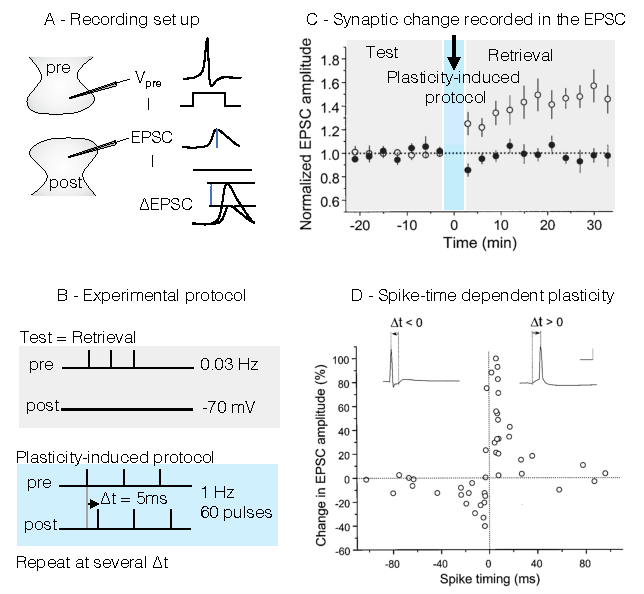
\includegraphics[scale=1]{latex/fig/Intro/SP_STDP.pdf}
    \caption{Caption \citep{bi_synaptic_1998}}
    \label{fig:SP_STDP}
\end{figure}

Figure \ref{fig:SP_Protocols} (top) provides an overview of the most common plasticity-induced protocols performed in the last years \citep{krieg_unifying_2014}. The strategy is to test the effect of one parameter onto the synaptic strength: such as the presynaptic frequency, the timelag between two pre and postsynaptic spikes ($\Delta t$), the postsynaptic membrane voltage $V_{\mathrm{post}}$ among others.
\begin{itemize}
    \item  the \textit{rate protocol} records the synaptic strength after exciting the presynaptic neuron at a given frequency while the postsynaptic is resting ($ \Delta w =F(f_{\mathrm{pre}}) $) \citep{dudek_homosynaptic_1992, frey_synaptic_1998, gerstner_hebbian_2011}.
    \item The \textit{Spike-Time Dependent Plasticity} protocol is largely used; the pre- and postsynaptic neurons are stimulated a low frequency (0.1 or 1Hz) with a certain timelag $\Delta t$ ($\Delta w =F(\Delta t$) \citep{debanne_asynchronous_1994, bi_synaptic_1998, markram_regulation_1997, abbott_synaptic_2000, gerstner_neuronal_1996}.
    \item The membrane \textit{voltage} of the postsynaptic neuron is affected the result of the rate-protocol ($\Delta w =F(V_{post}, f_{pre}$) \citep{bi_synaptic_1998, artola_different_1990, sjostrom_rate_2001, ngezahayo_synaptic_2000, artola_long-term_1993}.
     The \textit{frequency}-dependent protocol consists in generating spikes at a given pairing frequency ($f_{pairing})$  with presynaptic spikes preceding postsynaptic spikes by 10 ms (or post-pre with a time delay written -10 ms) ($\Delta w =F(f_{pairing}$ with $\Delta t = \pm 10 $ms)\citep{sjostrom_rate_2001}.
     \item \textit{More complex} induction protocols were designed. Triplet and quadruplets are similar as the STDP protocol, three or four spikes are generated instead of two have \citep{wang_coactivation_2005, froemke_spike-timing-dependent_2002, froemke_contribution_2006, wittenberg_malleability_2006}. Postsynaptic 'bursts':  repetitive action potentials in a short period of time of 1, 2 or 3 spikes paired with one single presynaptic spike induced experimentally in the cortex \citep{nevian_spine_2006, debanne_asynchronous_1994,froemke_contribution_2006}.
\end{itemize}
More details on plasticity induced protocols are available in \citep{inglebert_synaptic_2021, krieg_unifying_2014}. More factors can influence the result of the synaptic plasticity such as the synaptic location \citep{froemke_spike-timing-dependent_2002, sjostrom_cooperative_2006} and more indirect factors such at the initial synaptic strength \citep{ngezahayo_synaptic_2000}. 

\begin{figure}[h!]
    \centering
    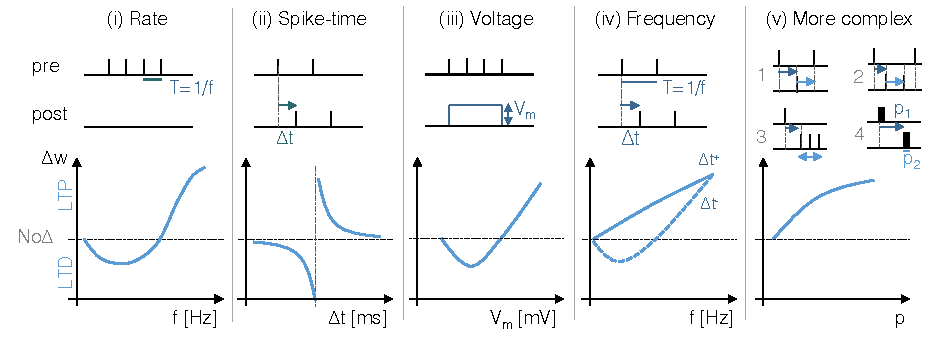
\includegraphics[scale=0.9]{latex/fig/Intro/SP_Protocols.pdf}
    \caption{Caption}
    \label{fig:SP_Protocols}
\end{figure}



\subsubsection{Short-term plasticity}
Short-term plasticity refers to changes in the synaptic transmission that occurs over a period ranging from miliseconds to several minutes. There are two types of short-term plasticity: facilitation and depression. Briefly, \textit{facilitation} involves an increase in the synaptic strength due to the rapid succession of action potentials at the presynaptic neuron \citep{castro-alamancos_distinct_1997}  This activity leads a buildup of residual calcium, which in turn  affects the exocytosis of synaptic vesicles resulting, in the change in probability of the neurotransmitter release \citep{citri_synaptic_2008}. In contrast, \textit{depression} involves a decrease of the synaptic strength caused by the depletion of neurotransmitter stores at the presynaptic terminal \citep{heidelberger_synaptic_2014}.

Short-term plasticity is often correlated with mechanisms at the presynaptic neurons while longer changes in the synaptic plasticity preferentially occur at the postsynaptic neuron. 



\subsubsection{Long-term plasticity: definition and classification}
\acrfull{LTP} was shown experimentally (exactly 50~years ago) by\citep{bliss_long-lasting_1973} as a long-term increase in the synaptic strength following a brief, high-frequency stimulation or other induction protocol \citep{baltaci_molecular_2019}. Nowadays, we define \acrshort{LTP} more globally as activity-dependent long-lasting increase in the synaptic strength \citep{abraham_is_2019, citri_synaptic_2008}. Fourty years ago,  \acrshort{LTP} was already divided into two categories depending on the generation of new proteins or not as shown experimentally in  \citep{frey_effects_1993, krug_anisomycin_1984} by using inhibitor of protein-synthesis.

\begin{itemize}
    \item \acrfull{E-LTP} refers to the early phase of long-term change, which is independent of protein synthesis, without any structural of the synapse. It lasts up to 1-3h.
    \item \acrfull{L-LTP} refers to the late phase, which is dependent on de-novo protein synthesis (with the activation of transcription factors) and structural change of the synapse.
\end{itemize}
Conversely, the concept of \acrfull{LTD} refers to long-lasting decrease in the synaptic strength. In the quest of unrevealing the mechanisms behind these long-term changes, the causal steps of the induction and the maintenance are recalled. It starts with the calcium influx inside the postsynaptic neuron that will trigger a signalling cascade. I will dissect this cascade to identify how plasticity occurs. 



\color{black}
~\\

\subsubsection{Mechanisms of early long-term potentiation (E-LTP) and depression (E-LTD)}
We need to zoom at the molecular level to understand the machinery.  Calcium enter the postsynaptic neuron and binds to calmodulin, forming the complex known as \acrfull{CaM}. This complex acts as a dynamic calcium sensor, depending on the concentration, it triggers differ processes that either lead to \acrfull{LTP} (for elevated calcium influx) or \acrfull{LTD} (for intermediate calcium influx) \citep{kotaleski_modelling_2010, feldman_spike-timing_2012, seibt_primed_2019}. Figure \ref{fig:SP_E-LTP} details their mechanisms. 

~\\
\textit{\acrfull{E-LTP}}\\
In the case of elevated  calcium influx, the calcium/calmodulin (CaM) complex triggers calcium/calmodulin dependent protein kinase, known as CaMK (see Figure \ref{fig:SP_E-LTP}A). A \textit{kinase protein} has the property to regulate other proteins by attaching phosphate groups, a process known as phosphorylation, which causes functional change in the targeted protein \citep{bear_neuroscience_2016, seibt_primed_2019}. In the context of synaptic plasticity,  CaMKII, a member of the CaMK family,  is known to phosphorylate a variety of proteins, including ion channels, neurotransmitter receptors, and synaptic scaffolding proteins. One of its most important targets is the \acrshort{AMPAr}. As previously explained, it is the primary mediator of fast excitatory synaptic transmission in the brain. Elevated calcium influx quickly activates CaMKII, which potentiates the synapse by two manners: 
\begin{itemize}
    \item (i) increase in existing \acrshort{AMPAr} efficiency via phosphorylation leading to a better synaptic transmission.
    \item (ii) insertion of new \acrshort{AMPAr} into the postsynaptic membrane - a process known as fast AMPAr trafficking.  Indeed, some vesicles queue near the membrane, and in response to \acrshort{CaMKII} activation, the vesicles filled with new \acrshort{AMPAr} fuse with the membrane and deliver new \acrshort{AMPAr} to the synapse, via exocytosis, causing the swelling of the spines \citep{seibt_primed_2019}.  
\end{itemize}
The \acrfull{E-LTP} is independent on de novo protein synthesis and morphological change of the spine. 

\begin{figure}[h!]
    \centering
    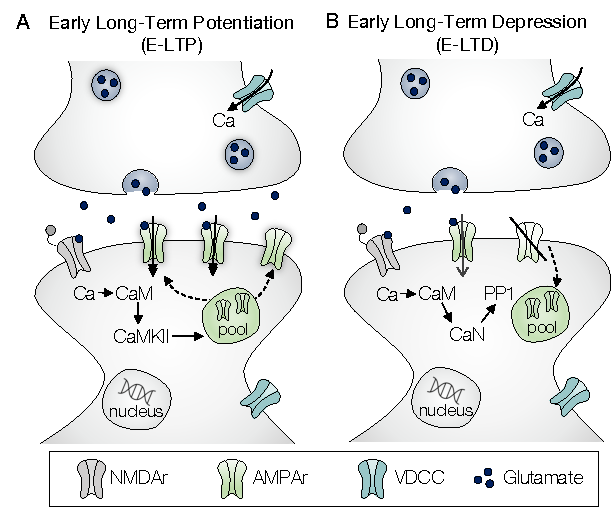
\includegraphics{latex/fig/Intro/SP_E-LTP.pdf}
    \caption{Caption}
    \label{fig:SP_E-LTP}
\end{figure}

~\\
\textit{\acrfull{E-LTD}}\\
In the case of intermediate calcium influx, the \acrfull{CaM} triggers calcium/calmodulin-dependent protein phosphatase, known as \acrfull{CaN} (see Figure \ref{fig:SP_E-LTP}B). A phosphatase protein is an enzyme that removes phosphatase from target proteins. This, in turn, activates another phosphatase protein called \acrfull{PP1}, which inhibits the action of CaMKII by dephosphorylating it \citep{citri_synaptic_2008}. 

As previously explained, calcium is crucial for synaptic plasticity, which raises the question of how a same signal can trigger \textit{both} LTP and LTD ? The key difference lies in the level of NMDAr activation, and it is important to remember that the different types of calcium response selectively activate different types of enzymes that have opossing effect. LTP and LTD reflect the bidirectional regulation of the phosphorylation and the number of AMPAr. \\ 



\subsubsection{Mechanisms of late long-term potentiation (L-LTP) and depression (L-LTD)}
The \acrshort{LTP} that lasts longer and induces changes in the spine morphology refers to \acrfull{L-LTP}. It is distinguished from \acrshort{E-LTP} by its protein synthesis. Figure~\ref{fig:SP_L-LTP} illustrates the mechanisms. 

On a longer timescale, the rise of calcium level that activates \acrshort{CaMKII} or CaMKIV (another member of the CaMK family) in turn activate \acrfull{cAMP} \citep{golbert_sleep_2017}. This  intracellular signaling molecule activates protein kinase A (pKA) (see Figure~\ref{fig:SP_L-LTP}A). Then, this latter enters the nucleus and activates transcription factors such as \acrfull{CREB} that regulates gene expression. These transcriptions factors can induce the expression of gene that encode new proteins, including \acrshort{AMPAr} and growth factors.  After the synthesis of new \acrshort{AMPAr}, they are trafficked to the synapse, via slow AMPAr trafficking. Additionally, the growth factors modify the synapse morphology and the cytoskeleton is impacted by modifying some support-protein such as \textit{actin}.  by Altogether, it contributes to the long-term morphological change such as for example enlargement of spine head (larger surface, increase in spine head volume, spine neck widening and shortening), growth of the dendtric spines (polymerization of actin filament), insertion of new receptors that were synthetized (by contrast to the fast trafficking of new receptors from the available vesicles pools), formation of new synapses, rearrangement of actin cytoskeleton and changes in the distribution of neurotransmitter receptors (receptor clustering).

Figure~\ref{fig:SP_L-LTP}B shows microscope imagine of a dendritic spine growth. The generation of new protrusions and the increase in volume of existing spines are clearly depicted \citep{lamprecht_structural_2004}.  The complementary process of \acrfull{L-LTD} triggers another signalling cascade that promotes the removal and inhibition of \acrshort{AMPAr} and the shrinkage of the spine \citep{bliss_long-term_2011}.

This level of details is sufficient for the purpose of my thesis for more information on the  intracellular signaling pathways see \citep{berridge_calcium_2014, citri_synaptic_2008, kotaleski_modelling_2010, bading_nuclear_2013, heidelberger_synaptic_2014,golbert_sleep_2017, seibt_primed_2019, feldman_spike_2020}.

\begin{figure}[h!]
    \centering
    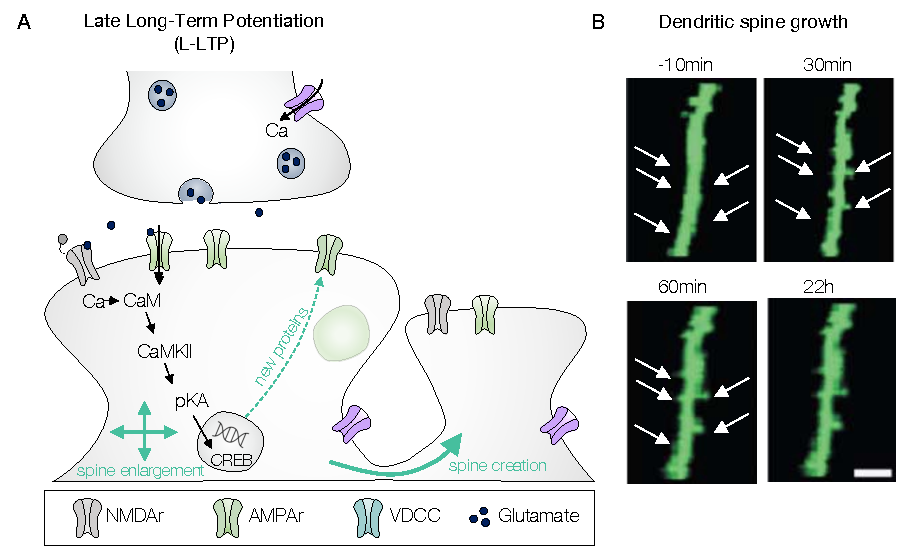
\includegraphics{latex/fig/Intro/SP_L-LTP.pdf}
    \caption{Caption \citep{lamprecht_structural_2004}}
    \label{fig:SP_L-LTP}
\end{figure}




\subsubsection{E-LTP, E-LTD, L-LTP, L-LTD, induction, expression, maintenance ... Clarificiation of the diverse concepts }

In my pursuit of understanding how neurons alter their connections with each other, I first reviewed synaptic transmission. Next, I distinguished between short-term and long-term changes, and then classified long-term changes into two categories based on the generation of new proteins: early and late processes. I also detailed the causal steps that mediate lasting changes at the synapse.

Figure \ref{fig:SP_Summary} presents a schematic overview of what I will refer to as \textit{traditional synaptic plasticity} and \textit{structural synaptic plasticity}. The terminology in this field can be overwhelming, but I aim to summarize the various concepts in a concise manner and present the hypothesis of my thesis.

The process known as \acrfull{E-LTP}, or \textit{LTP expression} \citep{heidelberger_synaptic_2014}, involves the exocytosis of new AMPAr from the vesicle pool and an increase in the efficacy of existing receptors, without any protein synthesis or spine morphological changes \citep{lamprecht_structural_2004}. In computational neuroscience, it is often associated with the \textit{traditional plasticity rule}.

In contrast, \acrfull{L-LTP}, or \textit{LTP maintenance} \citep{heidelberger_synaptic_2014}, involves an increase in the number of receptors in a given spine, changes in the efficacy of existing receptors, and even more characterizing of this phase, the morphological changes in the spine \citep{lamprecht_structural_2004}. The generation of new proteins mediates this process, and in computational neuroscience, it is often modeled by the \textit{structural plasticity rule}.

In both situations, \acrshort{AMPAr} are likely to be inserted or remove from the postsynaptic membranes but the insertion mechanism is different dependent the \acrshort{LTP} category. During \acrshort{E-LTP}, new receptors are inserted at the postsynaptic membrane from pools of available receptors. By contrast, for \acrshort{L-LTP}, the insertion of new receptors requires first its production thanks to protein synthesis. 

Many factors complicate our understanding of synaptic plasticity, such as presynaptic transmitter release or gene activation \citep{baltaci_molecular_2019, citri_synaptic_2008}. Neuromodulators are also likely to affect several factors in different ways. Further studies on plasticity at the molecular, neuronal, and population levels are necessary to gain a better understanding of learning and memory, and eventually provide guidance for related diseases.







\begin{figure}[h!]
    \centering
    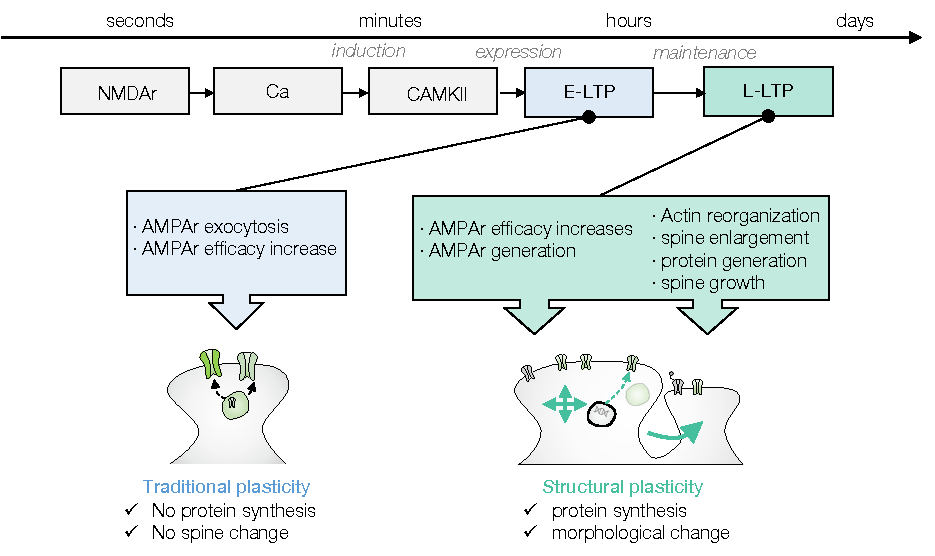
\includegraphics{latex/fig/Intro/SP_Summary.pdf}
    \caption{Caption}
    \label{fig:SP_Summary}
\end{figure}


\newpage
~\\
\newpage
\color{gray}
\subsection{Further mechanisms}

\textcolor{red}{PARAGR à rédiger à la fin  quand on conclu }
\subsubsection{Memory is dynamics}
To conclude this section on synaptic plasticity, it is important to note that memory is stored on synapses that are dynamically regulated. Ongoing plasticity of connections empowers animal and human to live, learn and react on a dynamic environment \citep{abraham_is_2019}. Additionally, there is more and more evidence that memory is not fixed forever on a given network, naming for example memory drift \textcolor{red}{REF}. Memory also involves consolidation between different brain regions as described in the theory of active memory consolidation \citep{born_sleep_2006}.

\subsubsection{Intrinsic plasticity}
Another type of synaptic plasticity really relevant at the circuit level is intrinsic synaptic plasticity \citep{daoudal_long-term_2003, debanne_plasticity_2019, sehgal_learning_2013}. It is defined as change in intrinsic property of a neuron like change in the number of density of ion channels.

bio: \citep{debanne_spike-timing_2010}

\subsubsection{Synaptic-Tagging and Capture Hypothesis}
This hypothesis proposes that only tagged synapses can used \acrfull{PRP} that are necessary for \acrshort{L-LTP} \citep{baltaci_molecular_2019, abraham_is_2019}.

\textcolor{red}{A voir si on laisse ici ou si on explique ca dans la review}


\subsection{NMOD OF SP}
\citep{frey_effects_1993} "L-LTPcome from thefindingthatL-LTPisblockedbyantag- onistsofdopaminereceptors"


"Modulatory neurotransmitters such as dopamine (DA), noradrenaline (NA), serotonin (5-HT) and acetylcholine (ACh), which act on their respective receptors to activate cAMP-dependent signaling in neurons,41-44 also play a role in regulating the longevity of synaptic plasticity. Broadly speaking these neurotransmitters serve as physiological effectors of reward, punishment, arousal and attention, all brain-states that modulate the longevity of memory."


article bio: \citep{lisman_neohebbian_2011, lerner_neuromodulatory_2011}\\
~\\


\color{black} 
\begin{comment}
\color{black}
\begin{wrapfigure}{r}{0.45\textwidth}
    \centering
    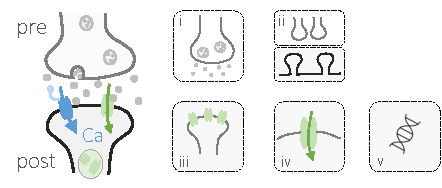
\includegraphics[scale=1]{fig/Intro/PlasticityType.pdf}
    \caption{\textit{Long-term synaptic plasticity expression.} \\
    \textcolor{cyan}{la figure est juste la pour montrer comment faire un wrap figure}
    \\In white boxes, changes concerning the presynaptic site. In light gray, changes concerning the postsynaptic site. From left to right: change in probability of neurotransmitter release, change in volume and number of dendritic spines, change in AMPA receptors number, change in receptor conductance and gene expression.  \textcolor{red}{adapter la légende + la figure sur base de Lamprechts 2004 super belle fig 1 + fig 2}}
    \label{fig:SP_PlasticityType}
\end{wrapfigure}
\end{comment}

\begin{comment}
\newpage
\color{gray}
\subsubsection{Vocabulary}

 memory engram \\
lire: \citep{choi_interrogating_2022} Recently, several studies verified the electrophysiological properties of the engram synapses. Engram synapses showed higher neuronal excitability and AMPA/NMDA ratio compared to other neurons [13,35]. If potentiation between engram cells had already occurred, it was difficult to have additional synaptic enhancements [36]. Even though the direct visual observation of synapses between the engram cells was not performed, it provided the physiological characteristics and functional changes of engram connections. Neuronal ensembles of engram cells distributed throughout the brain form functional neural networks [37, 38, 39]. Since the synapses that constitute this network eventually become the functional units that can subserve the functional roles of neurons, future investigations should incorporate the functional consequences with any interrogation of the physiological and structural relevance of such analyses.\\
\citep{} Memory formation and storage relies on structural changes that occur in the connectivity between neurons. Richard Semon, an early advocate of a physical theory of memory, was the first to term the neural substrate containing memories as the memory engram (Semon, 1904; Schacter, 2001). He defined the engram as the lasting modification produced by experience and stimulation in the brain. Attempts in the 20th century to find and identify the engram were intense\\
    GPT: A memory engram is a specific pattern of neural activity that represents a particular memory. It is thought that memories are encoded in the brain by creating specific engrams, which can be reactivated to retrieve the memory.\\
    ~\\
    \textit{Synapsogenesis} refers to the process by which new synapses are formed between neurons. %This process is critical for the development and plasticity of neural circuits, and it is believed to be a key mechanism underlying learning and memory.}

\color{black}
\end{comment}



 \begin{comment}
 >>> intro bien écrite pour un article 
 
\citep{choi_interrogating_2022}\\
 To form a network, neurons communicate with other neurons via synapses, and each synapse has its own functional properties depending on the presynaptic neurotransmitter and specificity of postsynaptic receptors. Various types of receptors are expressed at synapses in a neuron, indicating that multiple types of neurotransmitters are received as inputs – excitatory, inhibitory, or modulatory. As an example, amygdala pyramidal cells receive excitatory inputs from hippocampus and cortex, form inhibitory connections with neighboring interneurons, and even receive neuromodulatory inputs from the ventral tegmental area (dopamine) and dorsal raphe (serotonin) [9,22, 23, 24]. 
 (...) 

 The synapse, as the functional unit of neurons, is not a fixed structure, but rather undergoes constant changes by various stimuli. External stimuli activate neurons across the brain, and these activities induce structural/functional changes at the synapse, known as synaptic plasticity [25, 26, 27]. The most well-known functional synaptic plasticity is long-term potentiation (LTP), defined as persistence of synaptic strengthening, and is a key concept in learning and memory. LTP was first identified in the hippocampus in 1973 by Bliss and Lomo [28,29] and has since been verified by other methods through numerous studies thereafter [30,31]. This conserved principle has been extended to recent studies on engram cells, which have utilized diverse investigations of LTP in engram cells .

 \end{comment}


\begin{comment}
Just below,  the biological mechanisms underlying LTP and LTD are briefly described. The regulation of AMPAr are introduced such as their insertion or removal or their change in conductance \citep{bading_nuclear_2013, seibt_primed_2019, golbert_sleep_2017, berridge_calcium_2014}. NMDAr might also be dynamically regulated \citep{ferreira_co-agonists_2017}. The maintenance of the synaptic changes is explained by the change in gene expression and new proteins synthesis triggered by calcium signalling cascade \citep{halterman_neuroscience_2005, Korb_arc_2011}. The dendritic spines at the postsynaptic sites are likely to vary in volume and number \citep{segal_dendritic_2005, de_vivo_ultrastructural_2017}. This phenomenon is called \textit{structural plasticity}. Thanks to kinase signalisation, a late phase of plasticity can induce the production either of new synaptic contacts and/or growing of the spine (associated to LTP) or either pruning of old ones and/or shrinkage (associated to LTD). The strength of synaptic connection and volume of the dendritic spine seems to be linked \citep{bosch_structural_2012}. There are additional types of plasticity such as the one affecting \textit{presynaptic} site.  For example, the decrease or increase of neurotransmitter release also exist and are induced by calcium signalling as well. It has been demonstrated initially at hippocampal mossy fibers and cerebellar parallel fibers synapses but the list of other brain regions expressing this kind of presynaptic plasticity has grown \citep{yang_sleep_2014}.


Long-term changes in plasticity can be classified as either \textit{early-phase} or \textit{late-phase}, depending on whether the effects persist for several hours or longer \citep{citri_synaptic_2008}. The early-phase of plasticity transitions into the late phase as new proteins and ribonucleic acid messengers (mRNAs) are synthesized to support the maintenance of plastic changes \citep{bliss_long-term_2011}.
\end{comment}




\begin{comment}
\subsection{Computational model}
\textcolor{orange}{introduire la notion de w et décrire qu'il s'agit juste d'une équation différentielle qui va réguler w}

\subsection{Scale}
\textcolor{orange}{reprendre l'image de Christoph avec les différentes scales? }
\end{comment}

\newpage

% -------------------------
% -------------------------
%
%     NEUROMODULATION
%
% -------------------------
% -------------------------

\begin{comment}
\section{Neuromodulation}
\textcolor{orange}{avant la partie sur les switches ? }
\subsection{Concept}
\subsection{Neuronal}
\textbf{Biology}\\
~\\
\textbf{Modeling ! > si on fait dans le chapitre modeling autant tout mettre la }  
\end{comment}



% -------------------------
% -------------------------
%
%     RESEARCH QUESTION
%
% -------------------------
% -------------------------

%\section{Research question}
